\PassOptionsToPackage{table}{xcolor}
\documentclass[british,titlepage,oneside,page]{ntnuthesis}
\title{Implementation of a novel data driven and reference based compression strategy for trajectories}
\shorttitle{Implementation of a novel trajectory compression strategy}
\author{Lars Skifjeld}
\shortauthor{Lars Skifjeld}
\date{\ntnuthesisdate\space}

\addbibresource{thesis.bib}


% From https://www.overleaf.com/learn/latex/Glossaries

\makeglossaries % Prepare for adding glossary entries


\newglossaryentry{latex}
{
        name=latex,
        description={Is a mark up language specially suited for
                        scientific documents}
}

\newglossaryentry{bibliography}
{
        name=bibliography,
        plural=bibliographies,
        description={A list of the books referred to in a scholarly work,
                        typically printed as an appendix}
}

\newglossaryentry{maths}
{
        name=mathematics,
        description={Mathematics is what mathematicians do}
}


% --------------------
% ----- Acronyms -----
% --------------------

\newacronym{phd}{PhD}{philosophiae doctor}
\newacronym{CoPCSE}{CoPCSE@NTNU}{Community of Practice in Computer ScienceEducation at NTNU}
\newacronym{gcd}{GCD}{Greatest Common Divisor}
\newacronym{mrt}{MRT}{Matchable Reference Trajectory}
 % add glossary and acronym lists before document

\begin{document}

\chapter*{Abstract}

Geospatial data provides valuable insights into the movement patterns of entities and people. However, as the volume of this data continues to increase, storage and transmission become more challenging. Data compression is a common solution to this problem. In this thesis, we analyze a novel reference-based and data-driven trajectory compression algorithm, \textit{REST}. This algorithm utilizes the qualities of the dataset as a whole to effectively compress each trajectory. The results are promising, but using Dynamic Time Warping as a trajectory similarity measure requires significant computational resources. Therefore, we have developed a version that significantly improves performance. The method achieves a compression ratio of five and is nine times faster than the original algorithm. Furthermore, when comparing to non reference-based methods, the results indicate that REST has a much better runtime and compression ratio.

\chapter*{Sammendrag}

Geodata gir verdifull innsikt i bevegelsesmønstre for kjøretøy og mennesker. Ettersom mengden av denne typen data fortsetter å vokse, oppstår det utfordringer knyttet til lagring og overføring. En vanlig løsning er datakomprimering. I denne avhandlingen analyserer vi en ny referansebasert og datadreven komprimeringsalgoritme spesifikk for stidata, kalt \textit{REST}. Algoritmen utnytter datasettets karakteristikker for å effektivt komprimere hver enkelt sti. Resultatene er lovende, men det å bruke "Dynamic Time Warping" til stisammenligning er ressurskrevende. Derfor har vi utviklet en versjon som forbedrer kjøretiden. Denne oppnår en komprimeringsgrad på fem, samtidig som den er ni ganger raskere enn den opprinnelige algoritmen. Videre indikerer resultatene at REST, sammenlignet med andre ikke-referansebaserte metoder gir bedre resultater både med tanke på kjøretid og komp-rimeringsgrad.


\tableofcontents
\listoffigures
\listoftables
\lstlistoflistings

\printglossary[type=\acronymtype] % Print acronyms
\printglossary                    % Print glossary

\chapter{Introduction}
\section{Motivation}
% More and more spatial data -> compression methods for space saving -> in order to compress and to compare the quality of the compression we need trajectory similarity ( distance measure is a large part of compression )

In the era of digitilaztion more and more devices are generating data, in particular geodata, which is data containing the location of entities (like a car or a plane) and people. As well as sequences of locations which is known as trajectories. The sheer amount of data is challenging to handle because it is difficult to store and transmit. This data is useful in analysing movement patterns and gives insight in frequency of different paths.

A common approach to solve this is to compress the data, this means storing it with less space while containing most of the same information. There exists many different compression methods for all kinds of data not only geodata, however there has also emerged som compression methods specific for trajectories. For example PRESS, which compresses trajectories by representing them using trajectories from a subset of the data. This method is known as a "reference-based" approach. The quality of the subset is crucial, a good set has low redundancy and high coverage. \textcite{zhao2018rest} propsed another reference-based approach "REST" which is, according to the authors:
\begin{quote}
    "The first data-driven approach to compress trajectories in unconstrained space with both spatial and temporal dimensions considered."
\end{quote}
REST is a set of different methods which are all reference based and data driven. The different methods have different use cases, there are two main axes for the use cases: spatial-only/spatiotemporal and greedy/optimal. The results show REST outperforming other state of the art methods in terms of compression ratio, runtime and storage space. This is because of the inherent adaptability from data driven compression and the large space savings from a reference based approach.

In addition reference based compression provides another key advantage, namely being readable without decompression. This increases the usefulness of the compression. The need for decompression is a major disadvantage because it requires another step before the data is readable. This means more infrastructure to perform the decompression, as well as the resources used in the decompression, which can be a resource-intensive process.

\section{Research Questions}
%claim
In this paper we will implement a version of REST for spatial-only compression with two adjustments aimed at reducing the most intensive process in the algorithm, namely the trajectory distance measure. The first change reduces the amount of distance measures required by using a spatial filter. The second change is reducing the runtime complexity of the algorithm for trajectory distance by using an approximate value. We believe this can improve the runtime of REST and make it usefull in a big data setting.

In this paper we will compare the results from REST as propsed in \cite{zhao2018rest} and our version. As well as comparing REST to other state-of-the-art trajectroy compression methods in order to support or refute the results from \cite{zhao2018rest}. From this we derive the following research questions:

\begin{description}
    \item[RQ1] Does the suggested spatial filter improve the runtime of the original REST algorithm?
    \item[RQ2] Does the suggested approximation of the distance measure improve the runtime of the original REST algorithm without significantly worsening the precision?
    \item[RQ3] Does our implementation of the original REST outperform state of the art methods in terms of compression ratio and runtime?
    \item[RQ4] Does our implementation of the improved REST outperform state of the art methods in terms of compression ratio and runtime?
\end{description}

\section{Outline}
This thesis is a continuation of a project from the course \textit{TDT4151 - Computer Science, Specialization Project}. We do not assume that the reader is familiar with the project, so we will repeat the relevant findings in chapter 2 of this thesis. In addition, some sections have been expanded because they have become more relevant as the thesis took shape. This is specifically the section 2.1 "REST" and 2.4 "DTW" have been expanded. Here is the structure of this thesis:

Firstly \textbf{Chapter 2} is mostly based on the former report and summarizes relevant theory.
\newline
\textbf{\hyperref[chap:impl]{Chapter~\ref*{chap:impl}}} explains the specific implementation details of the REST algorithm. As well as a rundown of the different variants made.

For the source code for the algorithm and experiment setup see: github.com. To see the contribution made to the open-source rust library see:
% https://github.com/shshemi/dtw-rs/pull/1/files#diff-344ba2b71ffb93beac576f22ee219b4247385dd9b91f5f0b33ab583aab016427


\chapter{Background}
\label{chap:bg}

\section{Packed Hilbert R-tree}
\label{sec:rtree}
A Packed Hilbert R-tree is an extension of the R-tree, a balanced tree used for multidimensional data, in our case, spatial data. From \cite{rtree}, a regular R-tree stores all data as leaf nodes on the same level. All leaves have minimum bounding rectangles (MBRs) that geometrically contain the data element of that node. Parent nodes also have MBRs, MBRs of parents geoemtrically conatin all MBRs of the children. An example of this is shown in figure \ref{fig:rtree}, with the corresponding data in figure \ref{fig:mbrs}. This allows for efficient spatial queries. When querying with a spatial filter, the system will only explore nodes that have MBRs overlapping with the spatial filter. For large datasets, this can lead to significant performance gains for many queries, as much fewer nodes need to be accessed.

\begin{figure}
    \centering
    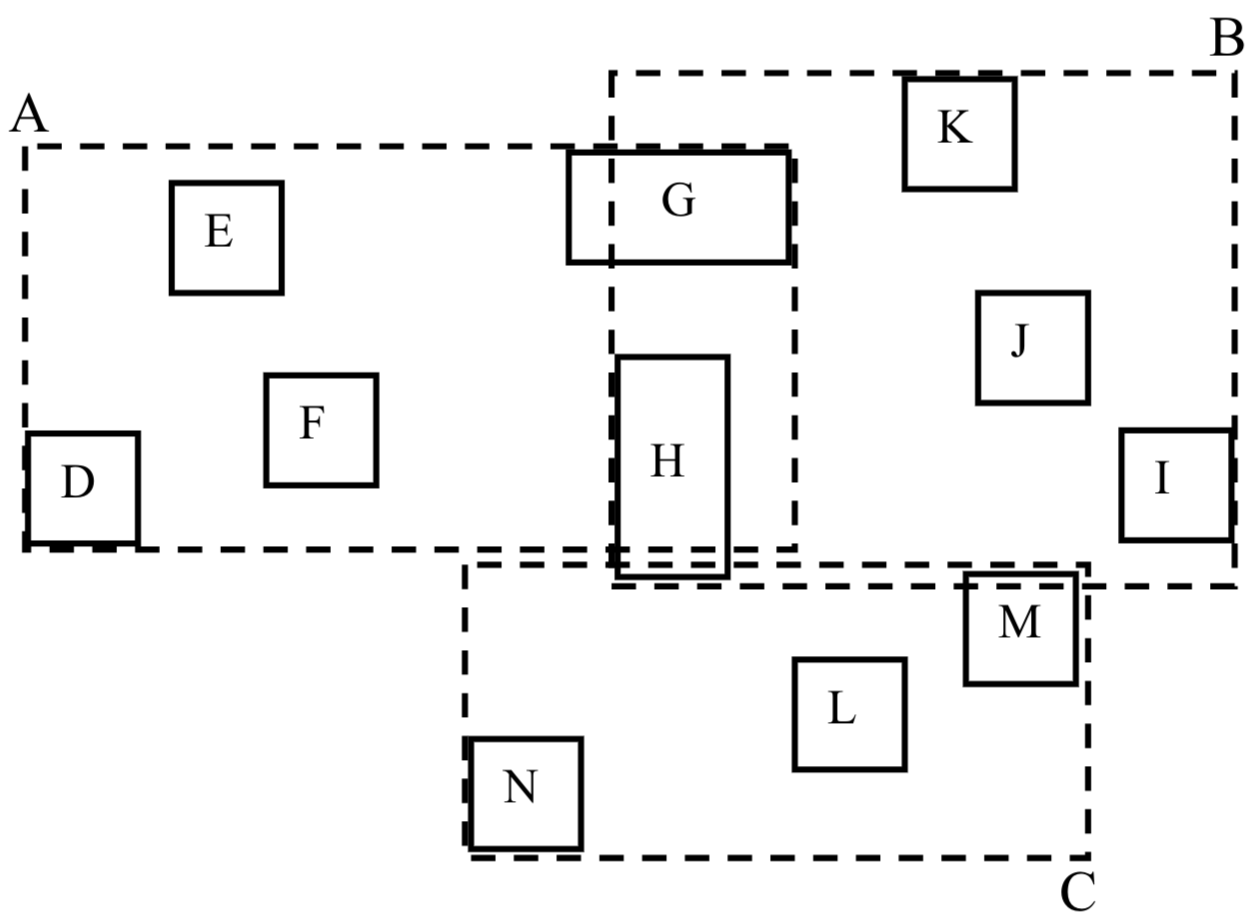
\includegraphics[width=0.5\linewidth]{./figures/mbrs.png}
    \caption{An example of data MBRs and their MBRs, from \cite{rtree}.}
    \label{fig:mbrs}
\end{figure}
\begin{figure}
    \centering
    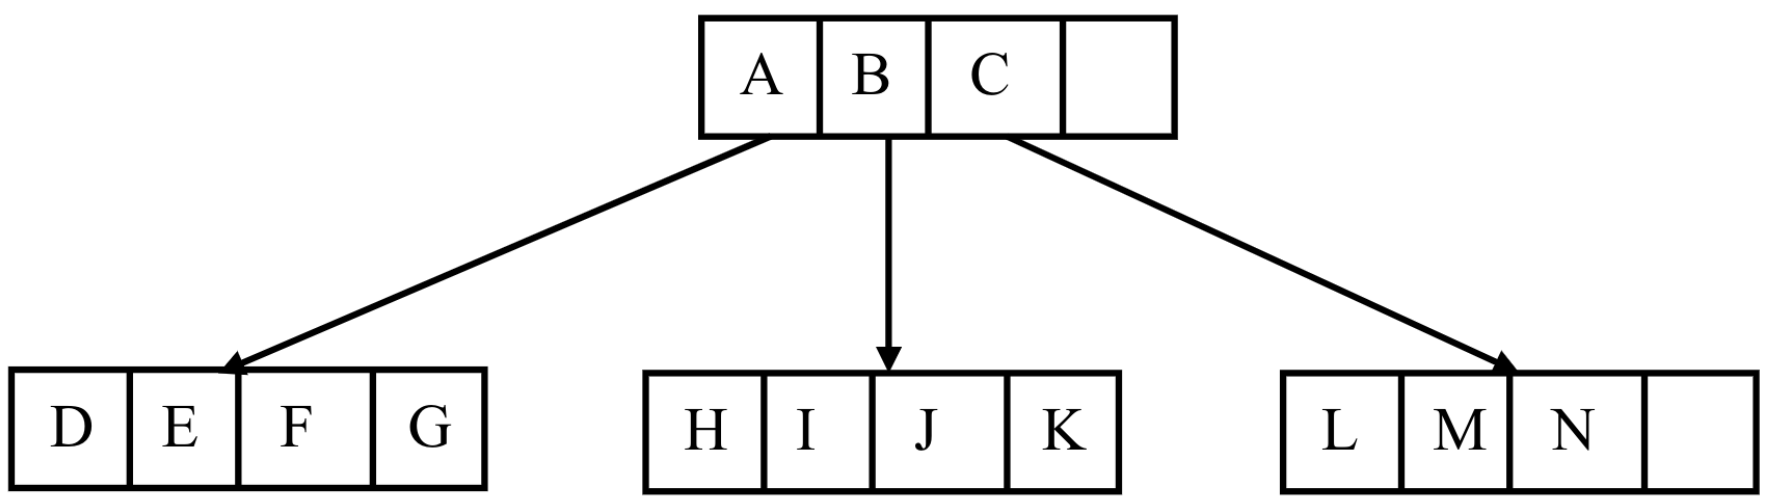
\includegraphics[width=\linewidth]{./figures/rtree.png}
    \caption{The corresponding R-tree, from \cite{rtree}.}
    \label{fig:rtree}
\end{figure}

What distinguishes a normal R-tree from a Hilbert R-tree is the MBR selection. The Hilbert R-tree utilizes Hilbert curves to generate MBRs for nodes. A Hilbert curve is a space-filling curve that can traverse every point in higher-dimensional space. This property allows for the mapping of two-dimensional values to one-dimensional values by drawing the curve in two dimensions and assigning ascending values to the points along the curve, see figure \ref{fig:hilbert} for Hilbert curves with corresponding values. These values are referred to as Hilbert values. Hilbert curves have the characteristic such that elements close in space will also be close in Hilbert values. By sorting MBRs based on the Hilbert value of the rectangle centroids, we can create MBRs with minimal overlap for spatial indexing.

\begin{figure}[t]
    \centering
    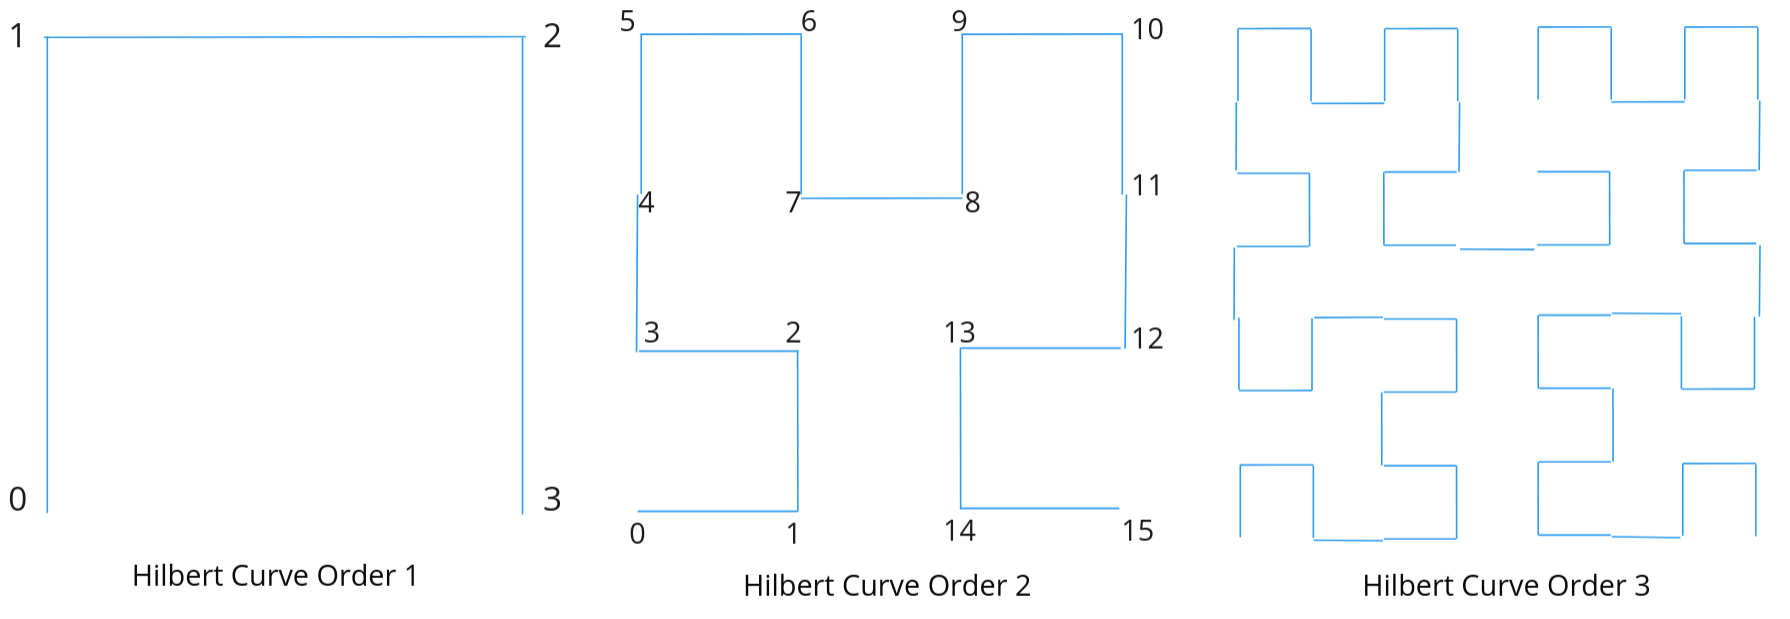
\includegraphics[width=\linewidth]{./figures/hilbert_orders.png}
    \caption{Showing Hilbert Curves of orders 1, 2, and 3.}
    \label{fig:hilbert}
\end{figure}

The Packed Hilbert R-tree is an optimized version of the Hilbert Tree. The Packed R-tree has even less overlap, resulting in improved query performance. The downside is that it requires more resources for construction. Considering the additional resource consumption, the Packed variant is only practical for applications that heavily prioritize read operations. In a system with frequent write operations, the entire tree would need to be rewritten frequently, leading to significant performance loss. For this reason, the Packed Hilbert R-tree is also known as the static Hilbert R-tree.
\section{Trajectory Compression}
\label{sec:traj}
\subsection{Methods in Trajectory Compression}
A trajectory is a sequence of geospatial points that represent a path, optionally including a timestamp. The goal of compression is to reduce the size of the trajectory by storing it in a compressed form while retaining the same information. This is measured using the compression ratio, which is the ratio between the uncompressed and compressed sizes and an accuracy metric. The accuracy metric determines to which degree information is retained. Furthermore, trajectory compression can be classified into three main categories: streamed/batched, lossless/lossy, and spatial-only/spatio-temporal.

The main difference between streamed and batched compression is the amount of data processed at a given time. Batched compression is generally simpler because it allows access to the entire trajectory at once. On the other hand, streamed compression can only handle one segment at a time due to memory limitations, which prevents the loading of the entire trajectory. This limitation complicates the process as the complete scope of the trajectory is unknown. A common approach to managing streamed data is the use of a Sliding Window, which forms the basis of many algorithms \cite{Sun2016}.

Batched compression, on the other hand, requires more storage and concentrated processing power. It necessitates loading the entire trajectory onto disk and processing it in a single operation. Due to its additional resource requirements and knowledge of the entire trajectory, batched compression outperforms streamed compression in terms of compression ratio and accuracy. Nonetheless, streamed compression can be advantageous in certain situations. Its ability to compress data as it is received, eliminating the need for intermediate storage, can outweigh the superior compression achieved by batched methods in terms of practicality. In addition, it is absolutely necessary for real time systems.

Lossy algorithms sacrifice accuracy for more efficient storage. Lossless algorithms reduce the size without losing any information. They generally have worse performance than lossy algorithms as a result of this. There is also category called \textit{Bounded Lossy Compression}, which was suggested by \textcite{zhao2018rest}. This allows compression algorithms to be lossy, but contained within an upper bound of "loss". The definition is stated by \textcite{zhao2018rest} as:

\begin{quote}
    \begin{definition}\label{def:bounded_lossy}
        Bounded Lossy Compression. Given a deviation $\epsilon$, an $\epsilon$-Bounded Lossy Compression algorithm transforms a raw trajectory $T$ into a compressed trajectory $T$, such that the distance between the reconstructed trajectory $T^*$ and $T$ does not exceed $\epsilon$, i.e., $d(T,T^*) \leq \epsilon$, where $d$ is some predefined distance function for trajectories.
    \end{definition}
\end{quote}

The distinction between spatial-only and spatio-temporal lies in the consideration of the temporal aspect, that is, whether time is taken into account or not. Spatial-only compression focuses solely on the spatial differences between trajectories. \textcite{SpatiotemporalComp}, define two spatio-temporal concepts that can improve trajectory compression: \textit{time-ratio distance} and \textit{speed difference threshold}.

The time-ratio distance represents the distance between two synchronized points: one point from the original trajectory and another point from the compressed trajectory. The traditional accuracy metric used in compression is the perpendicular distance between a point and the new trajectory. However, when using synchronized points the distance will change based on time. This was first defined by \textcite{SpatiotemporalComp} and has now been formalized as Synchronized Euclidean Distance (SED). Figure \ref{fig:sed} illustrates the concept of time-ratio distance, which will be further discussed in section \ref{subsub:SED}

The speed difference threshold is the concept of comparing speeds between sequential segments of the trajectory. The speed is not expected to be directly in the data; rather it is calculated as $ \Delta d / \Delta t $, where \textit{d} is distance and \textit{t} is time. When the speed difference is large this indicates a sudden movement or turn. These points are considered important for the internal shape of the trajectory. Therefore, ensuring no points with a speed difference larger than a certain threshold are removed during compression can increase the accuracy of the trajectory when considering the temporal aspect.

The results of the experiments by \textcite{SpatiotemporalComp} show that implementing a time-ratio distance and a speed difference threshold had a slight improvement in compression ratio and a significant reduction in error. Although the accuracy metric was spatio-temporal and the algorithms used for comparison were not, the results are not that surprising. Meanwhile, \textcite{Sun2016} claims that spatio-temporal compression is simple and efficient with the ability to maintain internal features in trajectories. However, they are unpopular because existing algorithms only consider speed which may lead to greater errors and break the holistic geometrical characteristics of trajectories.


\subsection{Accuracy Metrics}
The accuracy of compression can be measured using different metrics. This is done by calculating some distance between each point in the original trajectory and the new trajectory. Various operations can then be performed to obtain an overall metric. The mean distance of all points is the most commonly used measure, but other metrics such as median or maximum can also provide valuable insights into accuracy. The method used to calculate the distance, determines the accuracy metric. Example distances are shown in figure \ref{fig:sed}. The following sections will explore the most commonly used accuracy metrics, as mentioned by \textcite{TrajFramework} and \textcite{Sun2016}.

\subsubsection{Perpendicular Distance}
\label{subsec:PD}
Perpendicular distance (PD) refers to the shortest distance from a removed point to the new trajectory, as shown in figure \ref{fig:sed}. The shortest distance is always perpendicular to the trajectory, hence the name.

\subsubsection{Synchronized Euclidean Distance}
\label{subsub:SED}
SED is a measurement where a point $p_{i}$ is assigned a distance to the new trajectory that is equal to the distance to the synchronized point $p'_{i}$, as shown in figure \ref{fig:sed} $p'_{i}$ is calculated as:
\begin{equation}
    \begin{aligned}
        t'_{i} & = t_{i}                                                \\
        x'_{i} & = x_{s} + \frac{t_{i}-t_{s}}{t_{e}-t_{s}}(x_{e}-x_{s}) \\
        y'_{i} & = y_{s} + \frac{t_{i}-t_{s}}{t_{e}-t_{s}}(y_{e}-y_{s}) \\
    \end{aligned}
\end{equation}
This accuracy metric takes time into account. Two trajectories traversing the exact same spatial points might still be considered different if one took a longer time. This can be a useful metric for differentiating between taxi trips in rush hour and outside rush hour, since the trips outside rush hour will typically be shorter.

\begin{figure}[ht]
    \begin{minipage}[b]{0.49\linewidth}
        \centering
        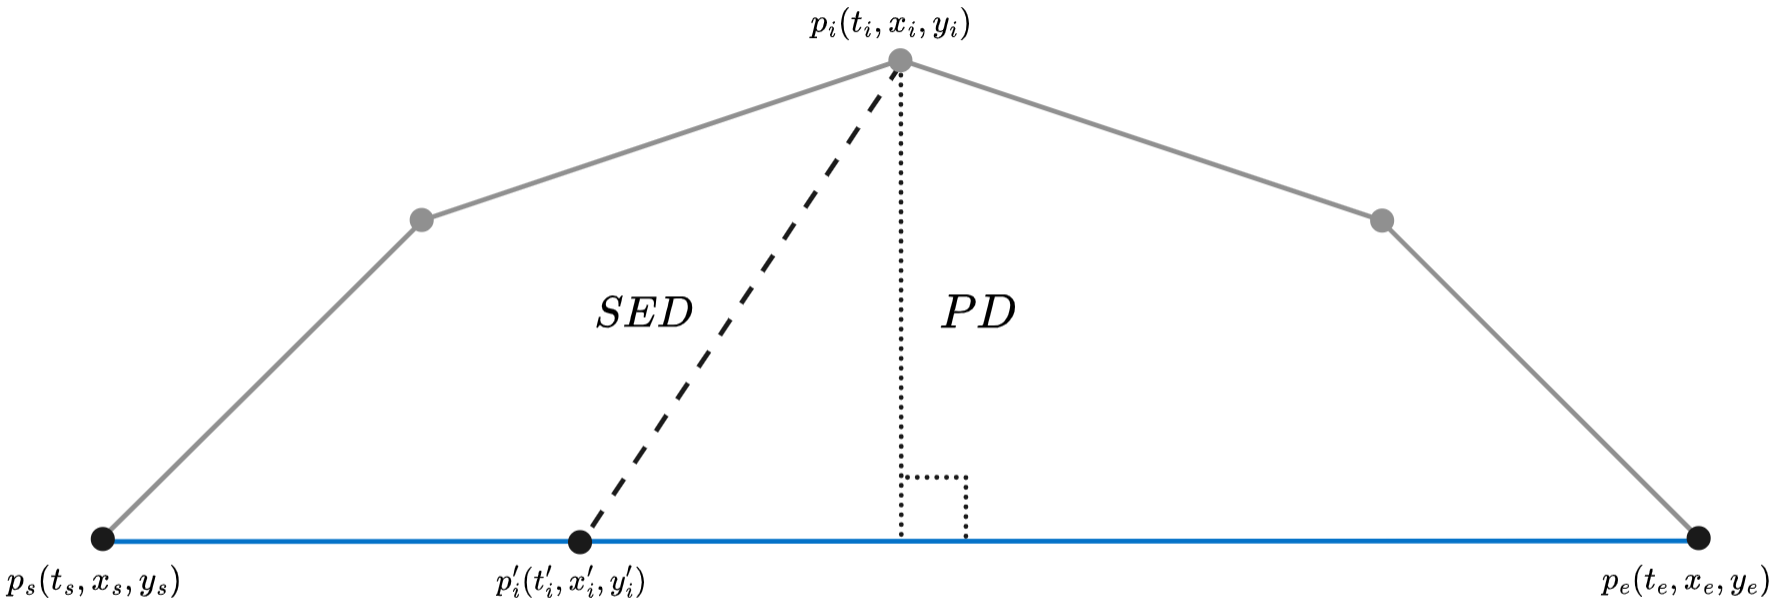
\includegraphics[width=\linewidth, height=7cm, keepaspectratio]{./figures/sed.png}
        \caption{Original trajectory in gray and new trajectory in blue showing distances SED and PD.}
        \label{fig:sed}
    \end{minipage}
    \begin{minipage}[b]{0.49\linewidth}
        \centering
        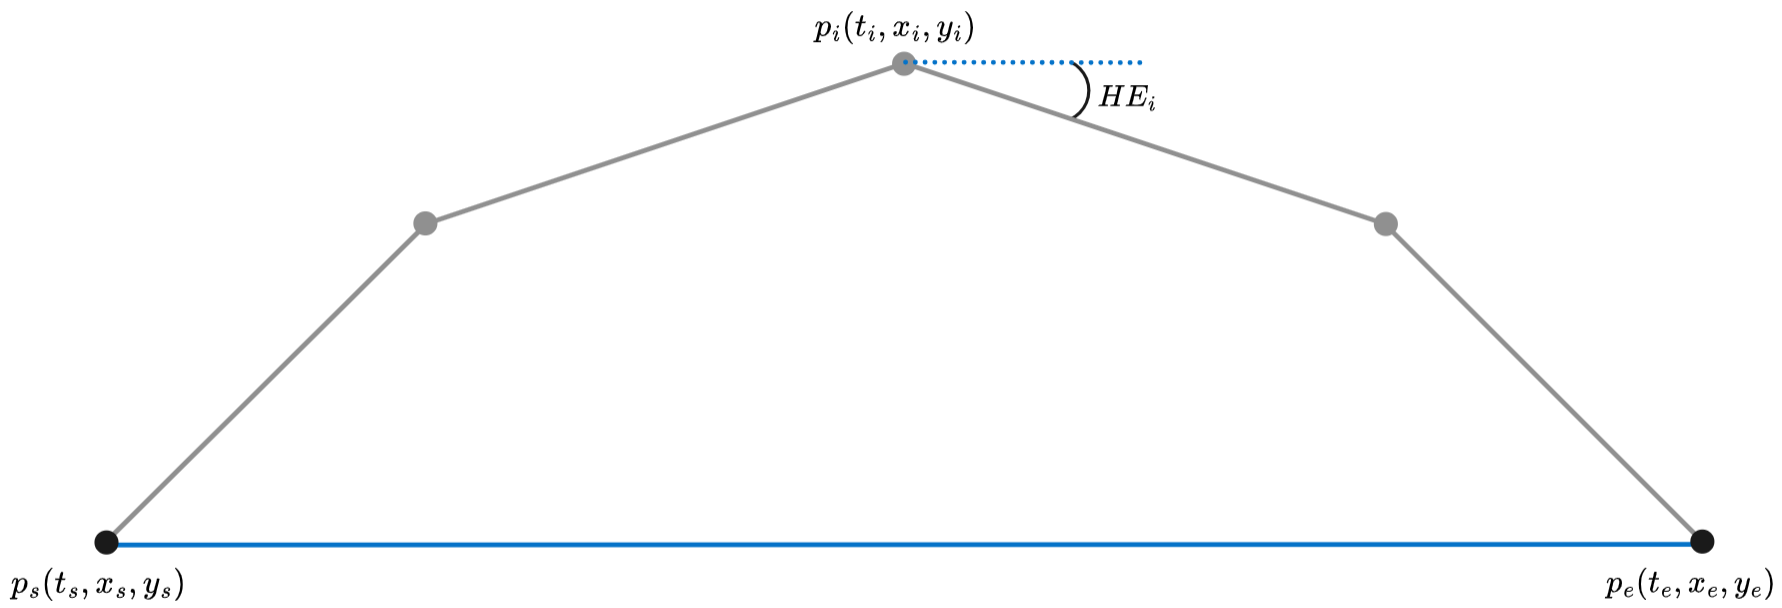
\includegraphics[width=\linewidth, height=7cm, keepaspectratio]{./figures/heading_error.png}
        \caption{Original trajectory in gray and new trajectory in blue showing distances HE.}
        \label{fig:hed}
    \end{minipage}
\end{figure}

\subsubsection{Heading Error}
The Heading Error (HE) for a point $p_{i}$ is the angular difference between the line segment $p_{i}$-$p_{i+1}$ along the original trajectory and $p'_{i}$-$p'_{i+1}$ along the compressed trajectory shown in figure \ref{fig:hed}. The angle represents the difference in direction between the original and the compressed trajectory at a given point. This metric is useful for detecting erratic movement and disruption of traffic flow according to \textcite{TrajFramework}.

\subsubsection{Speed Error}
The Speed Error is similar to the Heading Error in that it compares the segments from the original trajectory with the corresponding segment in the compressed trajectory. However, it compares speed instead of direction. The Speed Error is the difference in speed between the original and compressed trajectory at a given point.

\subsection{Performance Metrics}
%Skrive no her? intro
\subsubsection{Compression Ratio}
The compression ratio measures the amount of data that is compressed. This is calculated as $C_{r} = \frac{|o|}{|c|}$, where $C_{r}$ is the compression ratio, $|o|$ is the size of the original data, and $|c|$ is the size of the compressed data. Storing a 10 GB file with 5 GB gives a compression ratio of $10 / 5 = 2$, meaning it was stored using half the original size. This can also be written as a 2:1 compression ratio.

\subsubsection{Compression Performance}
Compression performance measures the speed of compression as well as resource usage. Compression speed is simply the time it takes to compress. Resource usage, however can be measured in a variety of ways, this depends on what kind of usage you want to measure, such as memory usage or CPU time. Computer executions like these may vary in performance, so it is important to measure the average over multiple runs when conducting an experiment, both for compression speed and resource usage. Additionally, it is important that when comparing compression performance, the measurements were taken in the same environment, meaning the experiment was executed on the same computer with the same version of the program. Otherwise, the results are not comparable.

\section{Dynamic Time Warping}
\label{sec:dtw}
According to \textcite{muller2007dynamic}, Dynamic Time Warping (DTW) is an algorithm used to determine the alignment cost between two temporal series. It can align the series by finding corresponding points between the series and finding the optimal alignment. The total alignment cost describes how similar the series are according to the DTW measure. When trying to align two different series, the alignment cost will be high, for two similar series, it will be low. Regarding trajectory compression, the alignment cost between a compressed trajectory and the original describes how similar they are, or how much information is preserved in the compressed form. A compression with high accuracy will have a low alignment cost.

There are many variations of DTW, that are made to speed up or otherwise improve it. We will begin by explaining Classical DTW from \textcite{muller2007dynamic}.

\subsection{Classical DTW}
Classical DTW works by calculating the cost matrix between two series. The cost $d_{i,j}$ in a matrix $D$ between the series $A$ and $B$ where \textit{distance} is a distance function between points, is given by:
\begin{equation}
    \label{eq:dtw}
    \begin{aligned}
        d_{i, j} & = distance(A_{i}, B_{j}) + \min \left\{ \begin{aligned}
                                                                & d_{i-1, j-1} \\
                                                                & d_{i-1, j}   \\
                                                                & d_{i, j-1}
                                                           \end{aligned} \right\}
    \end{aligned}
\end{equation}
\textcite{muller2007dynamic} introduces two terms, \textit{cost matrix} and \textit{accumulated cost matrix}. The cost matrix is a matrix of distances between all points in series $A$ and $B$, an example of a cost matrix is shown in figure \ref{fig:dtw_cost}. From the cost matrix, an accumulated cost matrix can be derived, each matrix cell contains the accumulated cost as defined in equation \ref{eq:dtw}. The accumulated cost matrix corresponding to the example in figure \ref{fig:dtw_cost} is shown in figure \ref{fig:dtw_acc_cost}. From equation \ref{eq:dtw} we see that the cost $d_{i, j}$ depends on the cost of previous points, for the first point $A_{1}$ and $B_{1}$ the previous points will not be defined. Therefore, a padding row and column is added: $d_{0,0} = 0$, $d_{1, 0}...d_{n, 0} = \infty$ and $d_{0, 1}...d_{0, m} = \infty$, this padding can be seen in figure \ref{fig:dtw_acc_cost}. The distance function depends on the type of data and the purpose of the DTW measure, Euclidean Distance or SED are common choices. The matrix cells are calculated one by one, from the top row, from left to right, using the cost function as described in equation \ref{eq:dtw}. Figure \ref{fig:dtw_acc_cost} shows an example of a DTW cost matrix for vectors $A = [8, 3, 7, 4, 3]$ and $B = [9, 5, 2, 6, 4]$. The total alignment cost is the accumulated cost in the final cell, $d_{5,5}$ in figure \ref{fig:dtw_acc_cost}, or more generally $d_{n,m}$.

Additionally, \textcite{muller2007dynamic} introduces the term \textit{warping path}, which is a sequence of points (matrix cells) in an accumulated cost matrix, that defines alignment between two sequences. If a warping path for $A$ and $B$ in the matrix $M$, includes $M_{1,2}$ this represents aligning point $A_1$ to $B_2$. The \textit{optimal warping path} is the warping path with the lowest total cost among all possible warping paths \cite{muller2007dynamic}. To find the optimal warping path, start from the last cell of the matrix and trace back to the first, selecting the paths with the lowest costs. If there are ties in cost, a predetermined set of priorities for different path directions (diagonal, horizontal, vertical) is used. Consequently, there can be multiple warping paths with the same minimal cost, but only one optimal warping path. Figure \ref{fig:dtw_acc_cost} shows the optimal warping path drawn in the accumulated cost matrix.

\begin{figure}[h!]
    \centering
    \begin{tabular}{|c|c|c|c|c|c|c|}
        \hline
        \multicolumn{1}{|c|}{\diagbox{$A_{i}$}{$B_{j}$}} &          & 9        & 5        & 2        & 6        & 4        \\ \hline
                                                         & 0        & $\infty$ & $\infty$ & $\infty$ & $\infty$ & $\infty$ \\ \hline
        8                                                & $\infty$ & 1        & 3        & 6        & 2        & 4        \\ \hline
        3                                                & $\infty$ & 6        & 2        & 1        & 3        & 1        \\ \hline
        7                                                & $\infty$ & 2        & 2        & 5        & 1        & 3        \\ \hline
        4                                                & $\infty$ & 5        & 1        & 2        & 2        & 0        \\ \hline
        3                                                & $\infty$ & 6        & 2        & 1        & 3        & 1        \\ \hline
    \end{tabular}
    \caption{The DTW cost Matrix $M$ between vectors $A = [8, 3, 7, 4, 3]$ and $B = [9, 5, 2, 6, 4]$. The distance function for these one dimensional points is simply the absolute value of the difference. The blue line shows the optimal path between the vectors.
    }
    \label{fig:dtw_cost}
\end{figure}
\begin{figure}[b!]
    \centering
    \begin{tabular}{|c|c|c|c|c|c|c|}
        \hline
        \multicolumn{1}{|c|}{\diagbox{$A_{i}$}{$B_{j}$}} &                    & 9        & 5                & 2                  & 6        & 4                  \\ \hline
                                                         & 0\tikzmark{start1} & $\infty$ & $\infty$         & $\infty$           & $\infty$ & $\infty$           \\ \hline
        8                                                & $\infty$           & 1        & 3                & $6$                & $2$      & $4$                \\ \hline
        3                                                & $\infty$           & 7        & 3\tikzmark{end1} & $4$\tikzmark{end2} & $5$      & $3$                \\ \hline
        7                                                & $\infty$           & 9        & 5                & $8$                & $5$      & $6$                \\ \hline
        4                                                & $\infty$           & 14       & 6                & $7$                & $7$      & $5$\tikzmark{end3} \\ \hline
        3                                                & $\infty$           & 20       & 8                & $7$                & $10$     & $6$\tikzmark{end4} \\ \hline
    \end{tabular}
    \caption{The DTW accumulated cost Matrix $M$ for vectors $A = [8, 3, 7, 4, 3]$ and $B = [9, 5, 2, 6, 4]$. The costs are based on the cost matrix in figure \ref{fig:dtw_cost}. The blue line shows the optimal path between the vectors. The optimal alignment from $A$ to $B$ is $[8\rightarrow9, 3\rightarrow(5, 2), 7\rightarrow6, 4\rightarrow4, 3\rightarrow4]$. The alignment cost (or DTW distance) is the value in the last matrix cell, in this case $M_{5,5} = 6$.}
    \label{fig:dtw_acc_cost}
    \begin{tikzpicture}[overlay, remember picture]
        \draw[thick, blue, -, opacity=0.7] ($(pic cs:start1) + (0,-14.25)$) -- ($(pic cs:end1) + (0,-14.25)$);
        \draw[thick, blue, -, opacity=0.7] ($(pic cs:end1) + (0,-14.25)$) -- ($(pic cs:end2) + (0,-14.25)$);
        \draw[thick, blue, -, opacity=0.7] ($(pic cs:end2) + (0,-14.25)$) -- ($(pic cs:end3) + (-0.25,-14.25)$);
        \draw[thick, blue, -, opacity=0.7] ($(pic cs:end3) + (-0.25,-14.25)$) -- ($(pic cs:end4) + (-0.25,-14.25)$);
    \end{tikzpicture}
\end{figure}

\textcite{muller2007dynamic} discusses several ways to improve classical DTW, such as modifying the cost function to reduce the number of vertical and horizontal lines in the optimal path, thereby preventing the path from getting stuck on one sequence. One approach involves implementing lower weights for diagonal movements or altering the cost function to incorporate more of the previous points.

Additionally, \textcite{muller2007dynamic} describes techniques to speed up classical DTW by coarsening data or by using global constraints. Coarsening the data allows for an initial rough estimation of the optimal path, followed by a more precise calculation in the selected areas of the matrix. Global constraints, such as the Sakoe-Chiba band and the Itakura parallelogram eliminate parts of the matrix \cite{muller2007dynamic}. This requires less computation and ensures that the optimal path stays within some proximity to the main diagonal. The Sakoe-Chiba is discussed later in section 3.1.

One challenge with DTW is that distances varies with the length of the vectors. The distance between longer vectors tend to be greater than for shorter vectors. This happens because the total alignment cost adds up the costs for all previous points along the optimal path. Consequently, more points lead to a higher alignment cost even if the trajectories are very similar. To address this issue, normalized versions of DTW have been proposed, such as Average DTW and Max DTW \cite{zhao2018rest}. Max DTW in particular will be explained in the following section.

\subsection{Max DTW}
\textcite{zhao2018rest} introduced Max Dynamic Time Warping (Max DTW), a variant of classical DTW that accounts for the lengths of the vectors (trajectories). Max DTW changes the cost function by taking the max of the distance and the former points minimum instead of taking the sum like in equation \ref{eq:dtw}. The new cost function is
\begin{equation}
    \label{eq:max_dtw}
    \begin{aligned}
        d_{i, j} & = max(distance(A_{i}, B_{j}), \min \left\{ \begin{aligned}
                                                                   & d_{i-1, j-1} \\
                                                                   & d_{i-1, j}   \\
                                                                   & d_{i, j-1}
                                                              \end{aligned} \right\})
    \end{aligned}
\end{equation}
This new cost function does not accumulate like in classical DTW, it simply represents the worst alignment of the optimal path to the current cell. The final cost represents the highest cost for a single alignment along the optimal path for the vectors. An example of a Max DTW cost matrix is shown in figure \ref{fig:max_dtw}, the vectors $A$ and $B$ are the same as in figure \ref{fig:dtw_acc_cost}. Here we can see that the end $M_{5,5} = 2$, this represents the highest cost along the optimal path, which is aligning $A_2 = 3$ to $B_2 = 5$, the cost $|A_2 - B_2| = 2$ is also the total cost for the vectors when applying Max DTW.
\begin{figure}[b!]
    \centering
    \begin{tabular}{|c|c|c|c|c|c|c|}
        \hline
        \multicolumn{1}{|c|}{\diagbox{$A_{i}$}{$B_{j}$}} &                    & 9        & 5                & 2                  & 6        & 4                  \\ \hline
                                                         & 0\tikzmark{start1} & $\infty$ & $\infty$         & $\infty$           & $\infty$ & $\infty$           \\ \hline
        8                                                & $\infty$           & 1        & 3                & $6$                & $6$      & $6$                \\ \hline
        3                                                & $\infty$           & 6        & 2\tikzmark{end1} & $2$\tikzmark{end2} & $3$      & $3$                \\ \hline
        7                                                & $\infty$           & 6        & 2                & $5$                & $2$      & $3$                \\ \hline
        4                                                & $\infty$           & 6        & 2                & $2$                & $2$      & $2$\tikzmark{end3} \\ \hline
        3                                                & $\infty$           & 6        & 2                & $2$                & $3$      & $2$\tikzmark{end4} \\ \hline
    \end{tabular}
    \begin{tikzpicture}[overlay, remember picture]
        \draw[thick, blue, -, opacity=0.7] ($(pic cs:start1) + (0,-14.25)$) -- ($(pic cs:end1) + (0,-14.25)$);
        \draw[thick, blue, -, opacity=0.7] ($(pic cs:end1) + (0,-14.25)$) -- ($(pic cs:end2) + (0,-14.25)$);
        \draw[thick, blue, -, opacity=0.7] ($(pic cs:end2) + (0,-14.25)$) -- ($(pic cs:end3) + (-0.25,-14.25)$);
        \draw[thick, blue, -, opacity=0.7] ($(pic cs:end3) + (-0.25,-14.25)$) -- ($(pic cs:end4) + (-0.25,-14.25)$);
    \end{tikzpicture}
    \caption{The Max DTW accumulated cost matrix $M$ for vectors $A = [8, 3, 7, 4, 3]$ and $B = [9, 5, 2, 6, 4]$. The costs are based on the cost matrix in figure \ref{fig:dtw_cost}. The blue line shows the optimal path between the vectors. The optimal alignment from $A$ to $B$ is $[8\rightarrow9, 3\rightarrow(5, 2), 7\rightarrow6, 4\rightarrow4, 3\rightarrow4]$. The alignment cost (or Max DTW distance) is the value in the last matrix cell, in this case $M_{5,5} = 2$.
    }
    \label{fig:max_dtw}
\end{figure}

Max DTW is sensitive to outliers points because a single poor alignment can significantly increase the total alignment cost. Additionally, this measure does not indicate whether there are many points close to the alignment max or just one. This makes Max DTW most useful to test threshold conditions. For instance, an application where no point can have an alignment cost above a certain threshold. Max DTW is also normalized and can be used to compare distances for sequences of varying lengths.

\subsection{Sakoe-Chiba Band}
\label{sec:sakoe}
The Sakoe-Chiba Band was suggested by \textcite{sakoe1978dynamic} as a global constraint that restricts the matrix comparison area. This is not a specific DTW variant in itself, but is a simplification that can be applied to any DTW calculation. The accessible region of the matrix is a band drawn around the main diagonal. This can be seen in figure \ref{fig:dtw_band}, where the inaccessible area is gray.

This band reduces the runtime of the calculation, but also reduces the precision of the result. The band is centered around the diagonal and will therefore be most successful for series where the optimal warping path stays close to the diagonal \cite{sakoe1978dynamic}. This applies to series that are quite similar in length and location. Note that for series of dissimilar length the total cost will not necessarily be in $M_{n,m}$, but in the cell within the band size around the main diagonal that is closest to $M_{n,m}$. Distances in the matrix are calculated in Manhattan distance. As shown in Figure \ref{fig:dtw_band}, cells that are diagonal to the main diagonal do not fall within the band because their Manhattan distance from the main diagonal is two, while the band size is one.

\begin{figure}[h!]
    \centering
    \begin{tabular}{|c|c|c|c|c|c|c|}
        \hline
        \multicolumn{1}{|c|}{\diagbox{$A_{i}$}{$B_{j}$}} &                           & 9                   & 5                        & 2                         & 6                         & 4                         \\ \hline
                                                         & 0\tikzmark{start1}        & $\infty$            & $\infty$\cellcolor{gray} & $\infty$ \cellcolor{gray} & $\infty$ \cellcolor{gray} & $\infty$ \cellcolor{gray} \\ \hline
        8                                                & $\infty$                  & 1                   & 3                        & 6 \cellcolor{gray}        & 2 \cellcolor{gray}        & 4 \cellcolor{gray}        \\ \hline
        3                                                & $\infty$ \cellcolor{gray} & 7                   & 3\tikzmark{end1}         & $4$\tikzmark{end2}        & 5 \cellcolor{gray}        & 3 \cellcolor{gray}        \\ \hline
        7                                                & $\infty$ \cellcolor{gray} & 9 \cellcolor{gray}  & 5                        & $8$                       & $5$                       & 6 \cellcolor{gray}        \\ \hline
        4                                                & $\infty$ \cellcolor{gray} & 14 \cellcolor{gray} & 6 \cellcolor{gray}       & $7$                       & $7$                       & $5$\tikzmark{end3}        \\ \hline
        3                                                & $\infty$ \cellcolor{gray} & 20 \cellcolor{gray} & 8  \cellcolor{gray}      & 7 \cellcolor{gray}        & $10$                      & $6$\tikzmark{end4}        \\ \hline
    \end{tabular}
    \caption{The DTW accumulated cost Matrix $M$ for vectors $A = [8, 3, 7, 4, 3]$ and $B = [9, 5, 2, 6, 4]$ with a Sakoe-Chiba band of size 1 applied. The grey area is inaccessible for comparison. This can also be seen as setting the costs in the gray area to $\infty$.}
    \label{fig:dtw_band}
    \begin{tikzpicture}[overlay, remember picture]
        \draw[thick, blue, -, opacity=0.7] ($(pic cs:start1) + (-0.1,0.1)$) -- ($(pic cs:end1) + (-0.1,0.1)$);
        \draw[thick, blue, -, opacity=0.7] ($(pic cs:end1) + (-0.1,0.1)$) -- ($(pic cs:end2) + (-0.1,0.1)$);
        \draw[thick, blue, -, opacity=0.7] ($(pic cs:end2) + (-0.1,0.1)$) -- ($(pic cs:end3) + (-0.1,0.1)$);
        \draw[thick, blue, -, opacity=0.7] ($(pic cs:end3) + (-0.1,0.1)$) -- ($(pic cs:end4) + (-0.1,0.1)$);
    \end{tikzpicture}
\end{figure}
% J. Gudmundsson, J. Katajainen, D. Merrick, C. Ong, and T. Wolle, “Compressing spatio-temporal trajectories,” Computa- tional Geometry, vol. 42, no. 9, pp. 825–841, 2009.
% PRESS
% REST!!!
% SQUISH?
% GML?
% Douglas pecker
% Dead Reckoning
\section{Douglas-Peucker}
\textcite{dp} introduced the Douglas-Peucker (DP) line simplification algorithm. It is a Top-Down algorithm, which means it recursively partitions the line until some halting condition is met, from \cite{Sun2016}. DP begins by removing all points except for the end points, then it adds the point furthest from the line back into the graph. As this happens the line is updated to go through the newly added point. This process continues recursively by adding the point farthest from the line and updating the line until no point is further away than a certain threshold. See an example iteration of DP in figure \ref{dp}. The halting condition is met when no point is a further than the distance $d$ from the line.

DP's worst case runtime is $O(n^{2})$, however it is still used for its simplicity and efficiency in practice \cite{gudmundsson2009compressing}. Additionally, \textcite{gudmundsson2009compressing}, created an improved version which can run in $O(n\log(n))$ even in if the path is polygonal and self intersects. There are also implementations of DP that use spatio-temporal distance measures like SED.
\begin{figure}[h]
    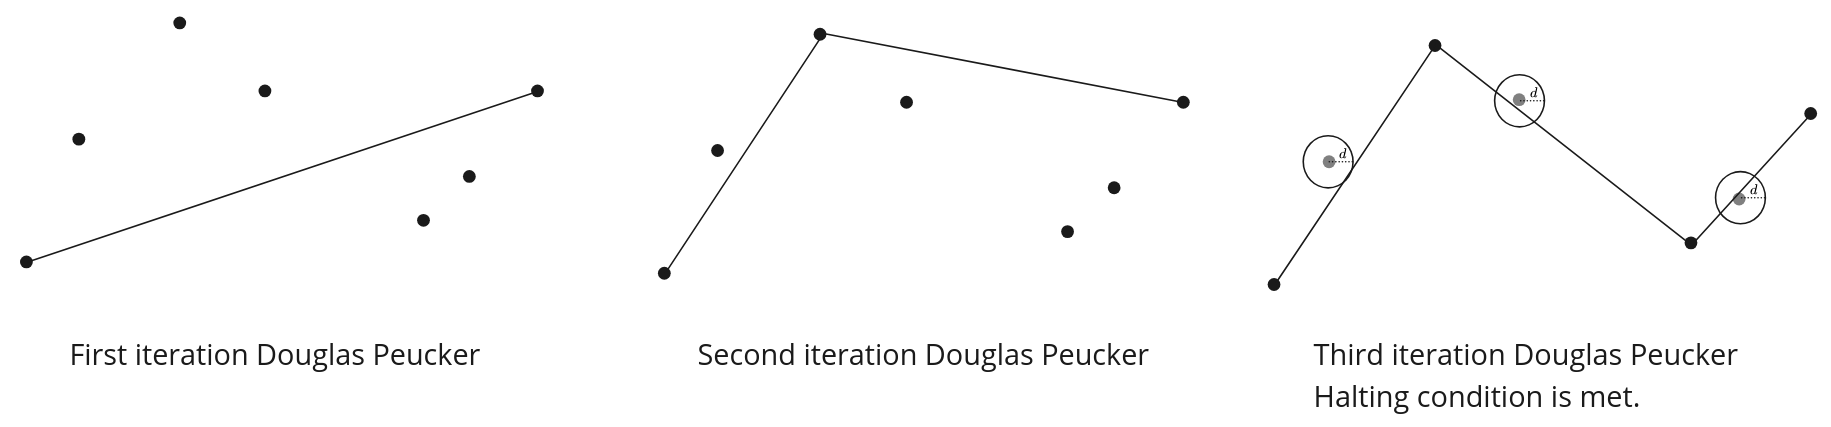
\includegraphics[width=1.0\linewidth]{./figures/dp.png}
    \caption{Three iteration of the Douglas Peucker algorithm, where the halting condition is met in the third iteration.}
    \label{dp}
\end{figure}

\section{SQUISH and SQUISH-E}
\textcite{muckell2011squish} introduced the Spatial QUalIty Simplification heuristic (SQUISH). It is a simple algorithm based on buffers and SED estimation. An input variable $\beta$ defines the buffer size. The algorithm sequentially loops through all the points in the trajectory; points are added to the buffer until it is filled. When a point is added the locally estimated SED error that would be introduced if the point is removed is calculated.

The first point is given an estimation of positive infinity, as it cannot be removed. When a point is added and the buffer is full, the point with the lowest estimated introduction of error is removed. This point is also referred to as the point with the highest priority. The introduction of error for its neighbors is then re-estimated. The neighbors contain some hidden information about the point that was removed, therefore the re-estimation will increase their estimated introduction of error. This process continues by removing the highest priority point in the buffer until all points have been processed. The result is a buffer filled with the points that represent the compressed trajectory. This algorithm has a run-time complexity of $O(n\log{\beta})$. It is important to note that the buffer size is static and defined as an input variable, which leads to predictable memory usage during execution.

In figure \ref{fig:squish} an example of the algorithm with a buffer size 4 is shown. The buffer is gradually filled up with points and their estimated introduction of error. When the buffer is full and point $E$ is processed, the highest priority point $B$ is removed. After removal, point $E$ is added and the error is re-estimated for $B$'s neighbors $A$ and $C$.

While this algorithm performs well compared to others when considering SED for small compression ratios, it has severe drawbacks such as the local estimations' incapability with large compression ratios. As a result, \textcite{muckell2014compression} introduced Spatial QUalIty Simplification Heuristic Extended (SQUISH-E), \raggedright an improved version of the original algorithm.
\begin{wrapfigure}[25]{r}{0.5\textwidth}
    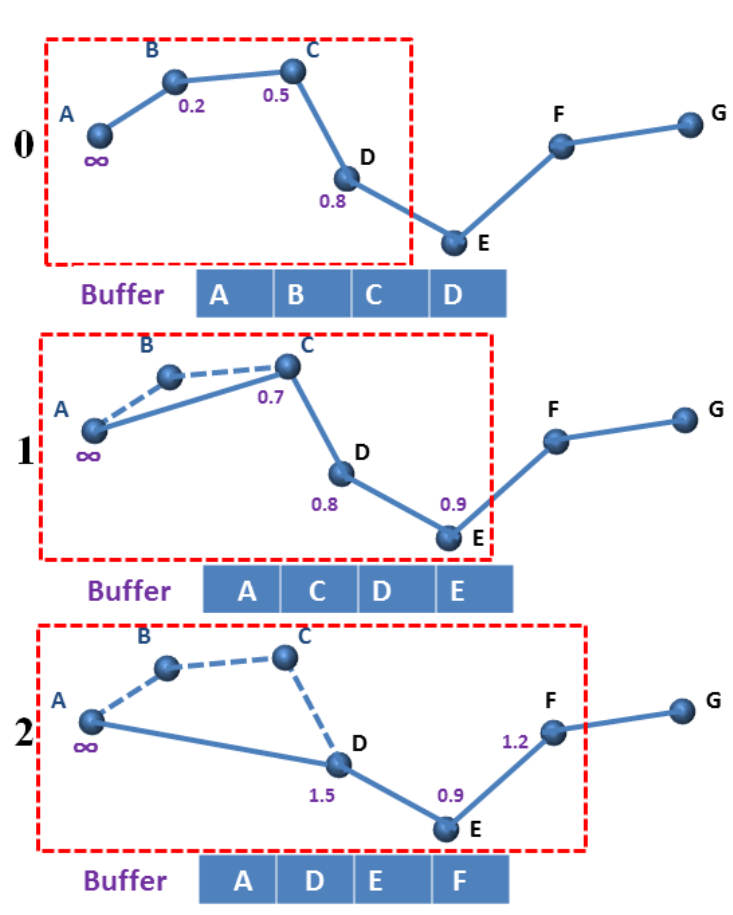
\includegraphics[width=0.5\textwidth]{./figures/squish.png}
    \caption{SQUISH estimates the lowest SED error
        and removes the point which is predicted to introduce
        the lowest amount of error into the compression. From, \cite{muckell2011squish}.}
    \label{fig:squish}
\end{wrapfigure}

The central change in SQUISH-E is a flexible buffer size combined with a maximum SED threshold. This change ensures that no point with an estimated SED over a certain threshold is removed, instead the buffer is expanded. The improved algorithm introduces two additional parameters: $\lambda$ and $\mu$. $\lambda$ represents the target compression ratio and $\mu$ represents the upper limit for SED error. Using these parameters, two modes are defined: SQUISH-E($\lambda$) and SQUISH-E($\mu$). In SQUISH-E($\lambda$), $\mu$ is set to zero, causing the algorithm to minimize SED error while ensuring a compression ratio of $\lambda$. On the other hand, SQUISH-E($\mu$) refers to the situation where $\lambda$ is set to 1. This will maximize the compression ratio while keeping SED error below $\mu$.

Experimental results from \textcite{muckell2014compression}, show that SQUISH-E provides low SED errors with a much faster run time than any of the alternatives. Additionally, the algorithm allows for control over both compression ratio and accuracy, providing flexibility that is not offered by other algorithms.

\section{PRESS}
\textcite{song2014press}, introduced the novel framework PRESS (\underline{P}aralleled \underline{R}oad-Network-Based Trajectory Compre\underline{ss}ion). PRESS compresses trajectories from road networks efficiently, using three key features to achieve this. Firstly it separates the spatial path and the temporal information when representing a trajectory. Secondly it introduces a lossless spatial compression algorithm called Hybrid Spatial Compression (HSC). Thirdly PRESS supports many common queries for location based services without decompression.

The reason to separate spatial and temporal information is to better exploit the road network in compression, this is essential for the HSC algorithm. HSC first compresses based on shortest paths. It has a map of all shortest paths from node $e_i$ to $e_j$, if the trajectory to compress is exactly like the shortest path from $e_i$ to $e_j$, it simply stores these nodes instead of the spatial information in the trajectories. This strategy is employed based on the assumption that people will often take the shortest path when traveling in a road network. Afterwards HSC compresses based on frequent sub-trajectory (FST) coding. It will represent the remaining trajectories as FST codes, giving the most frequent FSTs the shortest codes. This way huge amounts of space is saved, since a code is significantly smaller than a trajectory. In additional PRESS implements the Bounded Temporal Compression (BTC) algorithm. BTC tries to remove nodes from the trajectory without creating large temporal errors. To measure the error, two error metrics are used; Time Synchronous Network Distance (TSND) and Network Synchronous Time Distance (NSTD). TSND is the maximum distance between a trajectory $T$ and its compressed version $T'$. NSTD is the maximum time difference between a trajectory $T$ and its compressed version $T'$, see figure \ref{press_error}. The result is lossless spatial compression and bounded temporal compression, ensuring high quality compressed data.

\begin{figure}[t]
    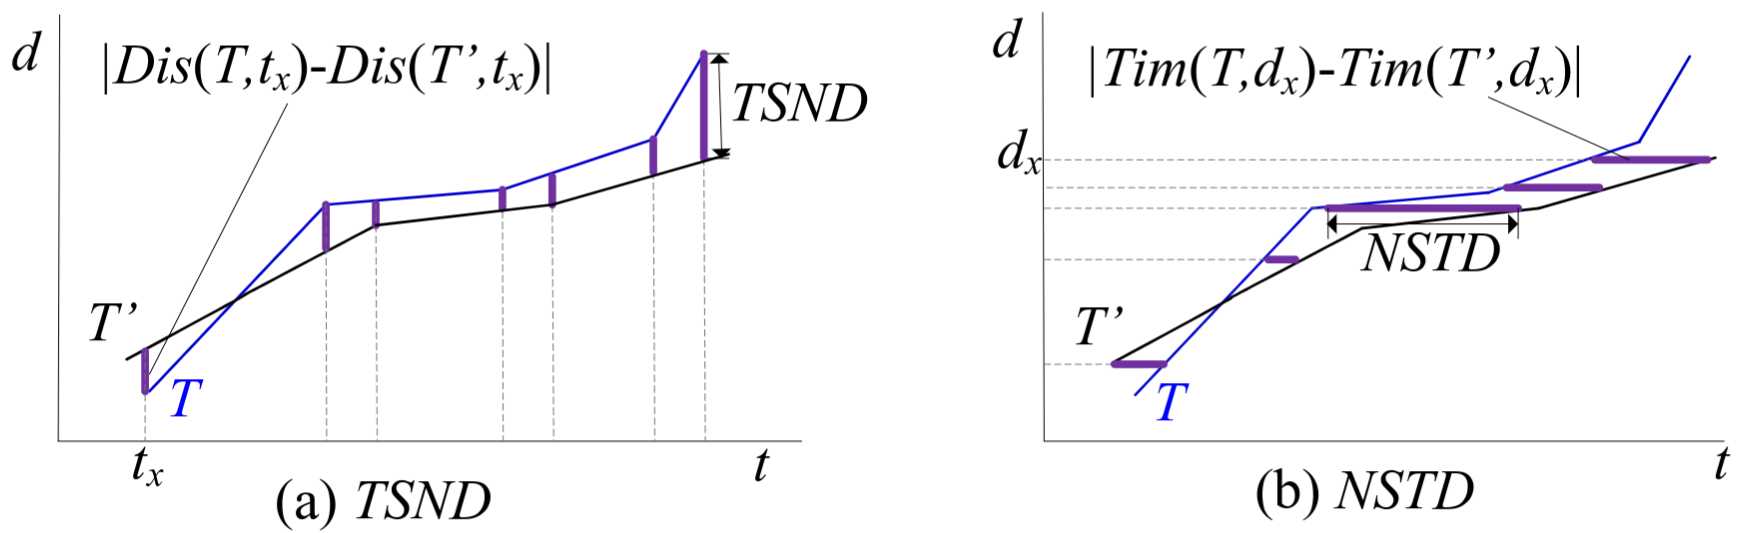
\includegraphics[width=1.0\linewidth]{./figures/press_error.png}
    \caption{TSND and NSTD, from \cite{song2014press}.}
    \label{press_error}
\end{figure}

The experimental results show that PRESS outperforms many competitors drastically in terms of compression ratio. PRESS was compared against two state-of-the-art approaches for trajectory compression in road networks. Map-matched trajectory compression (MMTCS) and Nonmaterial. When considering compression ratio we also need to define the error metric (aka, TSND and NSTD). With TSND and NSTD equal to 0, meaning no error tolerance, PRESS improved MMTC's compression ratio by 64\% and Nonmaterial's by 43\%. For TSED = 600 m, PRESS improved MMCTC's compression ratio by 280\% and Nonmaterial's by 199\%. These results show a significant improvement for compression ratio by a novel method.

\textcite{han2017compress} made a further improved version of PRESS called, COMPRESS (\underline{Com}prehensive \underline{P}aralleled \underline{R}oad-Network-Based Trajectory Compre\underline{ss}ion). This replaced the HSC part of PRESS with Hybrid Dictionary Compression (HDC) and Labeling and Coding (L\&C). COMPRESS is very similar to PRESS, but has multiple algorithms optimized for different data-types. Which makes it more applicable to multiple use cases.



\section{REST}
\label{sec:REST}
\textcite{zhao2018rest} introduced the REST (\underline{Re}ference-based \underline{S}patio-\underline{t}emporal trajectory compression) framework, which aims to efficiently represent raw trajectories by generating reference trajectories. The REST framework is categorized as bounded lossy compression. The objective is to minimize the error of the compression while using as few reference trajectories as possible. This approach is data driven, as it directly uses the raw trajectories to create the reference trajectory set.  Prior to REST, the only available data-driven method was PRESS. \textcite{zhao2018rest} mention some drawbacks of PRESS as motivation for creating the framework. One limitation of PRESS is that it limits trajectories to originate from a known road network. This can be problematic as there exists a large amount of unconstrained geospatial data. In addition, the algorithm needs updated road networks, which can be problematic due to frequent changes. However, REST has some similarities with PRESS in that reference trajectories are very similar to the frequent sub-trajectories (FSTs) in PRESS. The key difference is that reference trajectories in REST are unconstrained and data driven. While the FSTs in PRESS are partly data driven and constrained to a road network. This allows REST to be more easily generalized.

\begin{wrapfigure}[13]{r}{0.5\textwidth}
    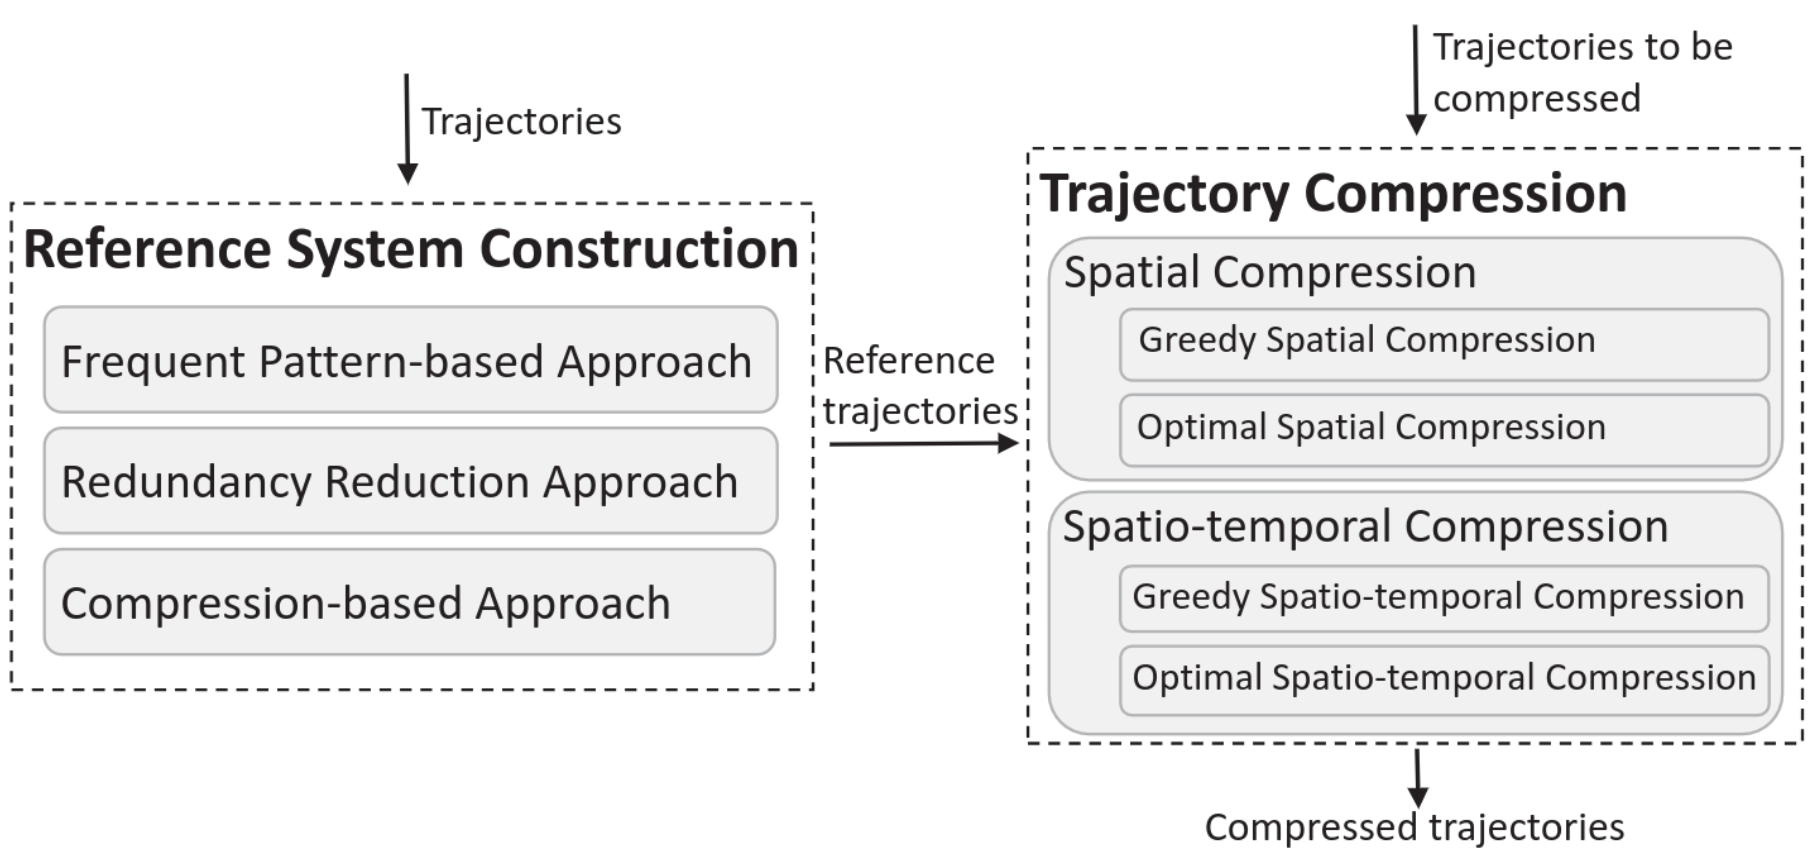
\includegraphics[width=0.5\textwidth]{./figures/rest_structure.png}
    \caption{REST framework overview, from \cite{zhao2018rest}.}
    \label{fig:rest_overview}
\end{wrapfigure}

Another motivation for creating REST was that existing trajectory compression frameworks like SQUISH, do not effectively utilize the characteristics of the entire trajectory set. SQUISH compresses trajectories individually in a vacuum, without considering their similarities. \textcite{zhao2018rest} also criticized SQUISH for assuming that moving objects do not frequently change speed and direction while traveling, which does not accurately represent real-world behavior. Consequently, algorithms like this cannot achieve high compression rates on real-world data. In contrast, data-driven compression such as REST, does not require such assumptions.

The structure of REST consists of two parts: the reference system construction and the compression of raw trajectories using the reference set, as seen in figure \ref*{fig:rest_overview}. Three methods were created for reference system construction; Frequent Pattern-based analysis, Redundancy reduction approach, and Compression-based approach. The methods attempt to create reference sets with high coverage and low redundancy. For the compression strategy, different methods were implemented in the categories spatial-only/spatio-temporal and greedy/optimal. Greedy Spatial Compression (GSC), Optimal Spatial Compression (OSC), Greedy Spatio-Temporal Compression (GSTC), and Optimal Spatio-Temporal Compression (OSTC). The greedy algorithms optimize locally instead of globally, therefore they are faster but with less accuracy than the optimal algorithms. The spatial-only algorithms only consider the spatial aspect which is simpler than the spatio-temporal aspect, they are both faster and more accurate (for spatial accuracy metrics).

From the experimental results, it was concluded that the Compression-based approach (CA) was the most effective. This approach compress training trajectories with the existing reference set and uses the compression ratio to interpret wheteher the training trajectory is reduntant or not. A high compression ratio indicates that the trajectory is redundant and should not be added to the reference set, a low compression ratio, on the other hand, indicates that the trajectory is not redundant and should be added to the reference set.

\begin{wrapfigure}[19]{r}{0.5\textwidth}
    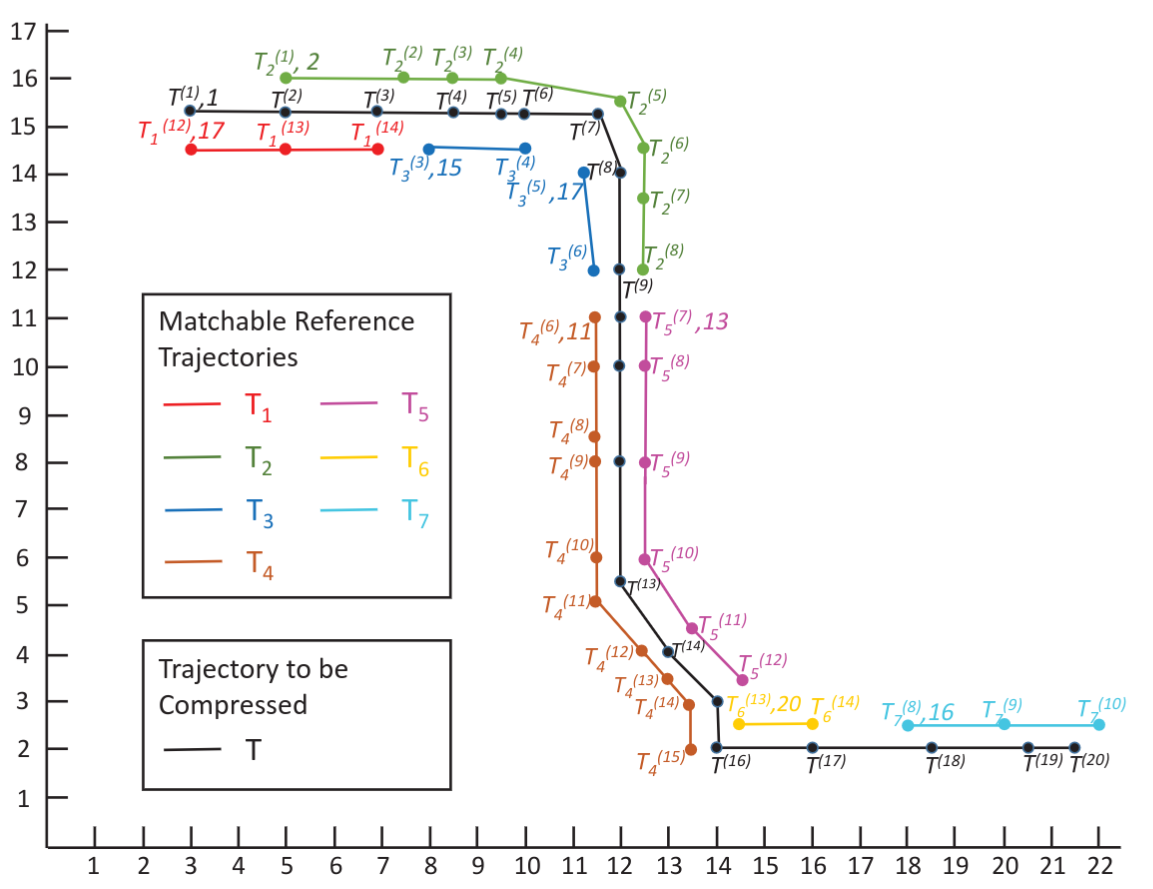
\includegraphics[width=0.5\textwidth]{./figures/rest.png}
    \caption{Matchable Reference Trajectories, from \cite{zhao2018rest}.}
    \label{fig:rest}
\end{wrapfigure}

In terms of trajectory compression, the results show that GSTC is preferred because it was the most well rounded algorithm. It was second most efficient (second to Douglas Peucker) and second to OSTC in accuracy. GSTC iteratively replaces the longest sub-trajectory with its Matchable Reference Trajectory (MRT). When selecting reference trajectory, GSTC selects the MRT that results in the lowest time correction cost. The time correction cost is defined as a variation of DTW, called MaxDTW. MaxDTW is different from DTW in that it looks at the maximum DTW across all pairs instead of the sum. In the figure \ref{fig:rest}, first $T^{(1,3)}$ is replaced by $T_1^{(12,14)}$, then $T^{(4,9)}$ is replaced by $T_2^{(3,8)}$, then $T^{(10,16)}$ is replaced by $T_4^{(6,15)}$, then $T^{(17)}$ remains in the compressed trajectory. The final segment $T^{(18,20)}$ is replaced by $T_7^{(8,10)}$

The results show that REST outperforms existing methods like PRESS and Douglas Peucker in terms of compression ratio and efficiency. One advantage of REST is that it is more flexible than existing methods, as it can be used in both constrained and non-constrained spaces. REST is also able to compress trajectories in spatial-only and spatio-temporal domains. The reference set can be stored using a much smaller storage space, as it is only a subset of all trajectories. Lastly the compressed data is simply a sequence of reference trajectories. This means that the compressed data is indexable and usable without computing any decompressed version. However, some memory lookup must be performed to retrieve the referenced trajectoryies. An index structure for this has not been implemented yet and is mentioned as future work.



\chapter{Related Work}
\label{chap:rel}
There is not much related work in this field, other than the original authors of REST expanding the original version with a Hybrid Index structure in order to query compressed trajectories. \textcite{zheng2019reference} suggest an IR-Tree as a Hybrid Index structure. An IR-tree is an R-tree based structure which provides document search and ranking for geodata \cite{li2010ir}. The following three features are a key part of the search: spatial filtering, textual filtering, and ranking. The filtering seeks to prune irrelevant nodes as early as possible, while the ranking attempts to provide the most relevant nodes first. The tree clusters nodes by their spatial data with textual data is stored as metadata.

This structure was efficient since the reference set is very small relative to the entire data set. Therefore the IR-tree was also small and can easily live in memory. The query processing showed promising results, outperforming state of the art methods.

Our work in this thesis differs from this in that the R-tree in our implementation is made before compression. It is created to speed up the building of the reference set and the compression afterwards. However, with some modifications, it can likely be used in a similar manner for querying after compression.
\chapter{Implementation}
\label{chap:impl}
This chapter explains the interpretation of REST that is implemented as well as different improvements that were made to speed it up. In this thesis we only look at spatial trajectory compression. In addition, the algorithms we selected from REST are the compression based approach to build reference set and the greedy spatial compression. This is because they showed promising results. Additionally, we explain how the DP-DTW comparison was made. This was coded in Rust and can be found on \href{https://github.com/Kilars/master-code/algo}{https://github.com/Kilars/master-code/algo}.


% In this chapter we will go through how the original version of REST as well as our variants were implemented. Without access to the source code we had to make assumptions for parts of the algorithm, in addition some smaller parts were changed from the original. The code for this algorithm was written in rust and the source code is available on "github.com". The chapter is divided into two sections, detailing the two different parts of the algorithm namely, reference set construction and the compression algorithm.
\section{REST}
In total there are 5 variants implemented. REST, REST\_EXCL, REST-SF, REST-BND, REST-KNN. All detailed in the following sections. The two following sections discuss the interpretation of REST for the compression based approach for reference set construction and the greedy spatial compression for the compression part.
\subsection{Reference Set Construction}
Reference set construction was implemented using the compression-based approach as defined by \textcite{zhao2018rest}, and introduced briefly in section \ref*{sec:REST}. This section will further discuss the reasoning behind the approach, as well as our method of implementation.

An efficient reference set has high \textit{coverage} with low redundancy, \textit{coverage} refers to the extent which the reference set represents the entire set of trajectories. A set with high coverage would yield a high compression ratio for all trajectories in the set. Redundancy refers to how much overlap there is between trajectories in the set. Striking a balance between coverage and redundancy is important, as too high coverage will likely lead to many trajectories in the set, leading to high redundancy. Conversely, tolerating too little redundancy will lead to too few trajectories in the set, resulting in insufficient coverage.

The compression-based approach naturally minimizes redundancy using the threshold and achieves sufficient coverage when using a large sample. It compresses a sample of all trajectories and adds those with compression ratios below a threshold to the set, indicating they are not well represented. The compression ratio threshold affects the redundancy tolerance; a lower threshold indicates a higher tolerance.

The pseudocode for this algorithm can be seen in code listing \ref{lst:ca_og}. The set is initialized as an empty list and trajectories are compressed and added or discarded iteratively. With a sufficient sample size the reference set will have high coverage for the entire set of trajectories.
\begin{figure}[t]
    \begin{lstlisting}[
        caption={Psuedo code for reference set construction},
        language=Pascal,
        label=lst:ca_og
    ]
        Input: T, rs
        Output: ReferenceSet
        ReferenceSet = []
        SampleTrajectorySet = AllTrajectories.take(10%)

        for ST in SampleTrajectorySet
            CR = Compress(ST, ReferenceSet)
            if CR < 5 
                ReferenceSet.add(ST)

        ReferenceSet
    \end{lstlisting}
\end{figure}

\subsection{Compression Algorithm}
For the compression algorithm we implemented Greedy Spatial Compression \break (GSC) from REST. This is an algorithm that searches greedily for the best result. It consists of two parts: a greedy match search and a wrapper connecting compression sequences of subtrajectories.
The matches are called Matchable Reference Trajectories and the definition is taken directly from \textcite{zhao2018rest}.
\begin{quote}
    Definition of Matchable Reference Trajectory (MRT). \textit{Given a sub-trajectory T(i,j) and a spatial deviation threshold $\epsilon_{s}$, its matchable reference trajectory set, denoted as M(T(i,j)), includes all the reference sub-trajectories with less-than-$\epsilon_{s}$ MaxDTW distance with T(i,j), i.e.,}
    \begin{align*}
        \hspace*{-3cm} M(T(i,j)) = \{ & \mathbb{T}(k,g) \mid \mathbb{T} \in \mathcal{R}, i \leq k \leq g \leq \left\lvert \mathbb{T} \right\rvert, \\
        \hspace*{-3cm}                & \text{MaxDTW}(T(i,j), \mathbb{T}(k,g)) \leq \epsilon_{s} \}
    \end{align*}
\end{quote}
From this and the properties of MaxDTW, \textcite{zhao2018rest} also derived a rule.

\begin{quote}
    \label{lemma}
    Lemma 1. \textit{Any sub-trajectory of the MRT of T(i, j) is also an MRT of sub-trajectory of T(i, j).}
\end{quote}

With the definition of an MRT and Lemma 1, the GSC algorithm can be explained.
For a trajectory \textit{T} = [$t_0$, ..., $t_n$] it searches for an MRT for the longest possible subtrajectory starting in $t_0$. If no \acrshort{mrt} is found then it adds [$t_0$, $t_1$] uncompressed to the compression sequence. Then it begins a new search starting in $t_1$. If an \acrshort{mrt} $r_{1,m}$ matches [$t_1$, ..., $t_m$], the \acrshort{mrt} is added to the compression sequence. The compression sequence for [$t_0$, ..., $t_m$] would be [$t_0$, $t_1$, $r_{1,m}$]. This process continues until a compression sequence for [$t_0$, ..., $t_n$] is calculated. The pseudocode for \textit{mrt\_search} is written in algorithm 1 of \textcite{zhao2018rest}. The Rust code of our version \textit{greedy\_mrt\_search} can be found in code listing \ref{lst:ca_expand}. The function's input and output is shown in line 1-6, it has 4 input parameters:

\begin{figure}
    \begin{lstlisting}[
        caption={Greedy MRT Search algorithm from source code written in Rust},
        language=Rust,
        label=lst:ca_expand,
        numbers=left
    ]
    fn greedy_mrt_search<'a>(
        candidate_reference_trajectories: &[&'a [Point]],
        st: &[Point],
        spatial_deviation: f64,
    ) -> Option<(usize, &'a [Point])> {
        let mut length_match_map = HashMap::new();
        for rt in candidate_reference_trajectories {
            let mut current_rt_matches: HashSet<(usize, usize)> = (0..rt.len() - 1)
                .into_iter()
                .filter(|&j|
                    dtw(&st[0..=1], &rt[j..=j + 1]) < spatial_deviation
                )
                .map(|j| (j, j + 1))
                .collect();
    
            let mut matched_st_len = 1;
            while !current_rt_matches.is_empty() {
                matched_st_len += 1;
                current_rt_matches.iter().next().map(|arbitrary_match| {
                    length_match_map
                        .entry(matched_st_len)
                        .or_insert_with(||
                            &rt[arbitrary_match.0..=arbitrary_match.1]
                        )
                });
                
                current_rt_matches = current_rt_matches
                    .iter()
                    .filter(|&(_, rt_end)|
                        (matched_st_len < st.len() - 1) && (*rt_end < rt.len() - 1)
                    )
                    .map(|&(rt_start, rt_end)| {
                        [
                            (rt_start, rt_end),
                            (rt_end, rt_end + 1),
                            (rt_start, rt_end + 1),
                        ]
                        .into_iter()
                        .filter(|&(s, e)| {
                            dtw(&st[..=matched_st_len], &rt[s..=e]) 
                            < spatial_deviation
                        })
                    })
                    .flatten()
                    .collect();
            }
        }
    
        length_match_map.into_iter().max_by_key(|&(k, _)| k)
    }
    \end{lstlisting}
\end{figure}

\begin{itemize}
    \item{\textit{t} - The trajectory being compressed}
    \item{\textit{candidate\_reference\_trajectories} - The reference trajectories used in compression}
    \item{\textit{spatial\_deviation} - The spatial deviation threshold for MRTs}
\end{itemize}

The output is a tuple (\textit{m}, $r_{0,m}$) or None. \textit{m} is the last index of the subtrajectory corresponding to the MRT. $r_{0,m}$ is the MRT itself. The compressed subtrajectory is given by \textit{t} and \textit{m} as [$t_0$, ..., $t_m$], the first index is always 0 because of the greedy search strategy. The compressed subtrajectory is the longest subtrajectory with an MRT from \textit{candidate\_reference\_trajectories}. None is returned if no MRTs were found.

Line 7 in code listing \ref{lst:ca_expand} is the start of the function and initializes a map for subtrajectory - MRT pairs (same structure as the output of the function). Line 8-47 is the code block for search in each reference trajectory \textit{rt}. It initializes \textit{current\_mrts} with all length two MRTs for [$t_0$, ..., $t_i$] where $i = 1$ (line 9-15). It does this by calculating the dtw distance between [$t_0$, $t_1$] and subtrajectories [$rt_j$, $rt_{j+1}$] for $j = 0, 1, ..., m-2$, where $m$ is the length of the $rt$. $current\_mrts$ is the collection of all subtrajectories with dtw distance lower than the $spatial\_deviation$. It follows from \hyperref[lemma]{Lemma 1} that this will be the basis for all MRTs. This is because DTW can never decrease the cost to a point later in the matrix.

The loop in line 17-47 uses $current\_mrts$ to find MRTs for $st_{i+1}$ = [$t_0$, ..., $t_{i+1}$] and stores MRTs to the global set (line 20-26). For each $rt$ = [$rt_0$, ..., $rt_m$] in $current\_mrts$ (matches for $st_i$), three expansions are tested for a match with $st_{i+1}$:
\begin{itemize}
    \item {[$rt_0$, ..., $rt_m$]}
    \item {[$rt_m$, ..., $rt_{m+1}$]}
    \item {[$rt_0$, ..., $rt_{m+1}$]}
\end{itemize}
This is in accordance with the expansion in the REST mrt\_search algorithm. This loop continues, increasing $i$ for each iteration, as long as an MRT can be found for $st_{i+1}$ or until $i+1 = |st|$. In addition, an arbitrary match from the $current\_mrts$ is added to the global map if no entry exists for $st_{i}$, for each iteration. When this loop finishes, the algorithm repeats the process for another reference trajectory. In the end, on line 50 the (ST, MRT) tuple for the longest ST from the global map is returned.

We have implemented this conceptually the same way as REST, but with some pruning and practical programming considerations. For example in our version all searching for one reference trajectory is completed the first time it is loaded to memory. This is opposed to the pseudocode of the REST algorithm which checks for MRT expansions in an arbitrary manner. In addition, the initialization process for MRTs is changed. Our version checks all length two subtrajectories from RT with the length two subtrajectory [$t_0$, $t_1$], because this is a greedy algorithm which begins in T[0]. While the version in REST finds all MRTs for $[t_i, t_{i+1}] \in T$. This difference is due to their version working for both greedy and optimal strategies. This simplification could only be made by specializing the function to only support a greedy search.

Regarding MRT selection when multiple are available, this was done arbitrarily. From the definition, an MRT has a DTW distance to the subtrajectory being compressed lower than the spatial deviation threshold. This means one reference trajectory can have a lower DTW distance than another, while both are considered MRTs. From this one could argue that the algorithm should select the MRT with the lowest distance. However, this implementation of REST applies bounded lossy compression, which means any result within the threshold is valid or "good enough". Therefore, no resources are spent locating the best MRT within the threshold, even though the resources required aren't large because the DTW distance is calculated anyway. If this were implemented, it could be considered "best effort bounded lossy compression". Comparing that to bounded lossy compression would be interesting, but it was not done due to time constrains. It is also likely that it wouldn't make a large difference because a reference trajectory with a significantly lower DTW distance could also match for a longer subtrajectory. This means that if there were multiple MRTs to select, they are likely close in DTW distance to the relevant subtrajectory. The way the reference trajectories expand and how this effects the DTW distance is further discussed in results and discussion. %DISCUSSION REFERENCE
\subsection{Exclusive REST}
One nuance of the reference set construction algorithm which should be discussed is that the entire trajectory is added to the reference set. A trajectory as a whole can be determined non-redundant, even if some subtrajectories are redundant. The algorithm could then add only the non-redundant parts of the trajectory. This would not be an expensive process as the trajectory has already been compressed and divided into references and points. However, from our interpretation of \cite{zhao2018rest} section 3.3 the trajectory in its entirety is added to the reference set. This impacts the reference set by adding more redundancy to the set. Meanwhile, it also leads to more coverage since more of the trajectories are added. Whereas an implementation which only adds the non-redundant parts would have less redundancy and lower coverage. %+ having shorter trajectories since they are "oppstykket".
In order to analyze the difference in these approaches both were implemented. The version adding the entire trajectory to the set is called REST, since this is interpreted as being the original implementation. While the other version only adding non-redundant parts of the trajectory to the set is called Exclusive REST (XREST).
\subsection{Spatial Filter}
% Set construction
The compression algorithm uses the reference set as a basis for compressing new trajectories. Searching through the entire set for each compression to find candidates to use as references is highly inefficient. Therefore we implement a spatial filter so that the compression algorithm only consideres reference trajectories that are close to the trajectory currently being compressed. The spatial filter is an R-tree containing each point of each trajectory in the reference set. A leaf node in the R-tree contains the position of the point and a tuple index \textit{(i, j)}, \textit{i} is the index of the point's parent trajectory and \textit{j} is the index to the point itself. The psuedo code for reference set construction with a spatial filter is shown in code listing \ref{lst:ca_sf}

%Compression, eh kinda same thing
The implementation of the spatial filter influences the input parameter \break \textit{candidate\_reference\_trajectories} for code listing \ref{lst:ca_expand}. With no spatial filter this input is simply all trajectories in the reference set. However, with a spatial filter the rtree selects only the trajectories close to the compressed one. It does this with a range query for latitude and longitude. The point itself is in the center of the range. This can be viewed as creating a box around the first point and selecting all points within the box. The box in our implementation is a square with the length of the sides as an input parameter. A larger square means more points are considered, which might lead to longer runtimes. While a smaller square will have less area coverage, but a faster runtime. More details on balancing coverage and performance can be found in the Results/Discussion section. %Reference results

Note that all points of the reference trajectories are indexed in the R-tree, as shown in \hyperref[lst:ca_sf]{Code Listing \ref{lst:ca_sf}} line 10-12. For reference trajectory $rt = [rt_0, ..., rt_m, ..., rt_n]$, where $rt_m$ is within the range query, $rt_{m,n} = [rt_m, ..., rt_n]$ can be considered as an MRT. As the reference set grows, using the R-tree becomes increasingly faster compared to checking the entire reference set, since more points are pruned.

After the reference set is built from a sample of all trajectories, it should be packed. This is because the data will not change and can be considered static. The Packed Hilbert R-tree would likely perform well in this case since it is simple and efficient with for low dimensionality. Additionally it has a very high storage utilization, which is beneficial if the size of the reference set is a concern. However, due to time constraints, this was not implemented. Nonetheless, the authors recommend exploring this as future work.
\begin{figure}
    \begin{lstlisting}[
        caption={Psuedocode for reference set construction with spatial filter},
        language=Pascal,
        label=lst:ca_sf,
        numbers=left
    ]
        Input: SampleTrajectories, CompressionThreshold
        Output: (ReferenceSet, RTree)
        ----------------------------------------
        ReferenceSet = []
        RTree = new RTree()

        for ST in SampleTrajectorySet
            CompressionRatio = Compress(ST, ReferenceSet)
            if CompressionRatio < CompressionThreshold 
                i = ReferenceSet.len()
                for (pt, j) in ST
                    RTree.insert(pt, (i, j))
                ReferenceSet.push(ST)

        (ReferenceSet, RTree)
    \end{lstlisting}
\end{figure}
\subsection{KNN}
Ye I did it
\section{MaxDTW}
MaxDTW has been implemented locally in Rust following the definitions in \ref{sec:dtw}. One important efficiency gain was through memoization of DTW solutions. \\ \textit{greedy\_mrt\_expand} in code listing \ref{lst:ca_expand}, expands with one point at a time, this is like adding one row and column to the DTW matrix. Without memoization, the entire matrix must be recalculated. However, with memoization, only the new column and row need to be calculated, using the previously computed accumulated cost matrix. Additionally an optional Sakoe-Chiba band was implemented like described in \ref{sec:sakoe}.

At one point, we considered using the external Rust library \textit{dtw\_rs} instead of a custom implementation. To prepare for this, we contributed to it by finishing the Sakoe-Chiba band implementation. However, due to the aforementioned memoization, which requires some state awareness from the local environment, integrating this library demanded too many modifications. Consequently, we decided to develop our own implementation. Although this contribution was not used in our final results, it is available here: \\ \href{https://github.com/shshemi/dtw-rs/pull/1/files}{https://github.com/shshemi/dtw-rs/pull/1/files}.

\section{Douglas Peucker DTW}
\section{Data Set}
% \input{chapters/3-structure.tex}
\chapter{Results}
\label{chap:res}
In this section we will present and discuss the results from the experiments on the REST implementation. The experiments were conducted on an Intel(R) Xeon(R) Gold 6426Y processor with 500 GB RAM.

The dataset used for these experiments is distributed by \textcite{porto} and consists of taxi routes in the city Porto over the course of one year. These routes are in the form of trajectories with latitude longitude points. In total there are 1.7M trajectories, for most experiments 100K are used, otherwise this will be explicitly stated. 100K is used in order to achieve a feasible runtime, however the methods applied can also be used for larger dataset.

\section{Reference Set Construction}
Firstly we will look at reference set construction, both in terms of performance and set size. The metrics \textit{Sample size} and \textit{Set size} is the sample size used to construct the reference set and resulting set size. \textit{REST} is the implementation of the original algorithm, while \textit{REST-SF} is the same implementation with a spatial filter. The window size is also indicated in the name, following SF. \textit{REST-SF30} indicates the square's side length in the range query in meters. A window size of 30 means a box of $30\times30m^2$ for r-tree range queries.

\begin{figure}[ht]
    \begin{minipage}[b]{0.99\linewidth}
        \centering
        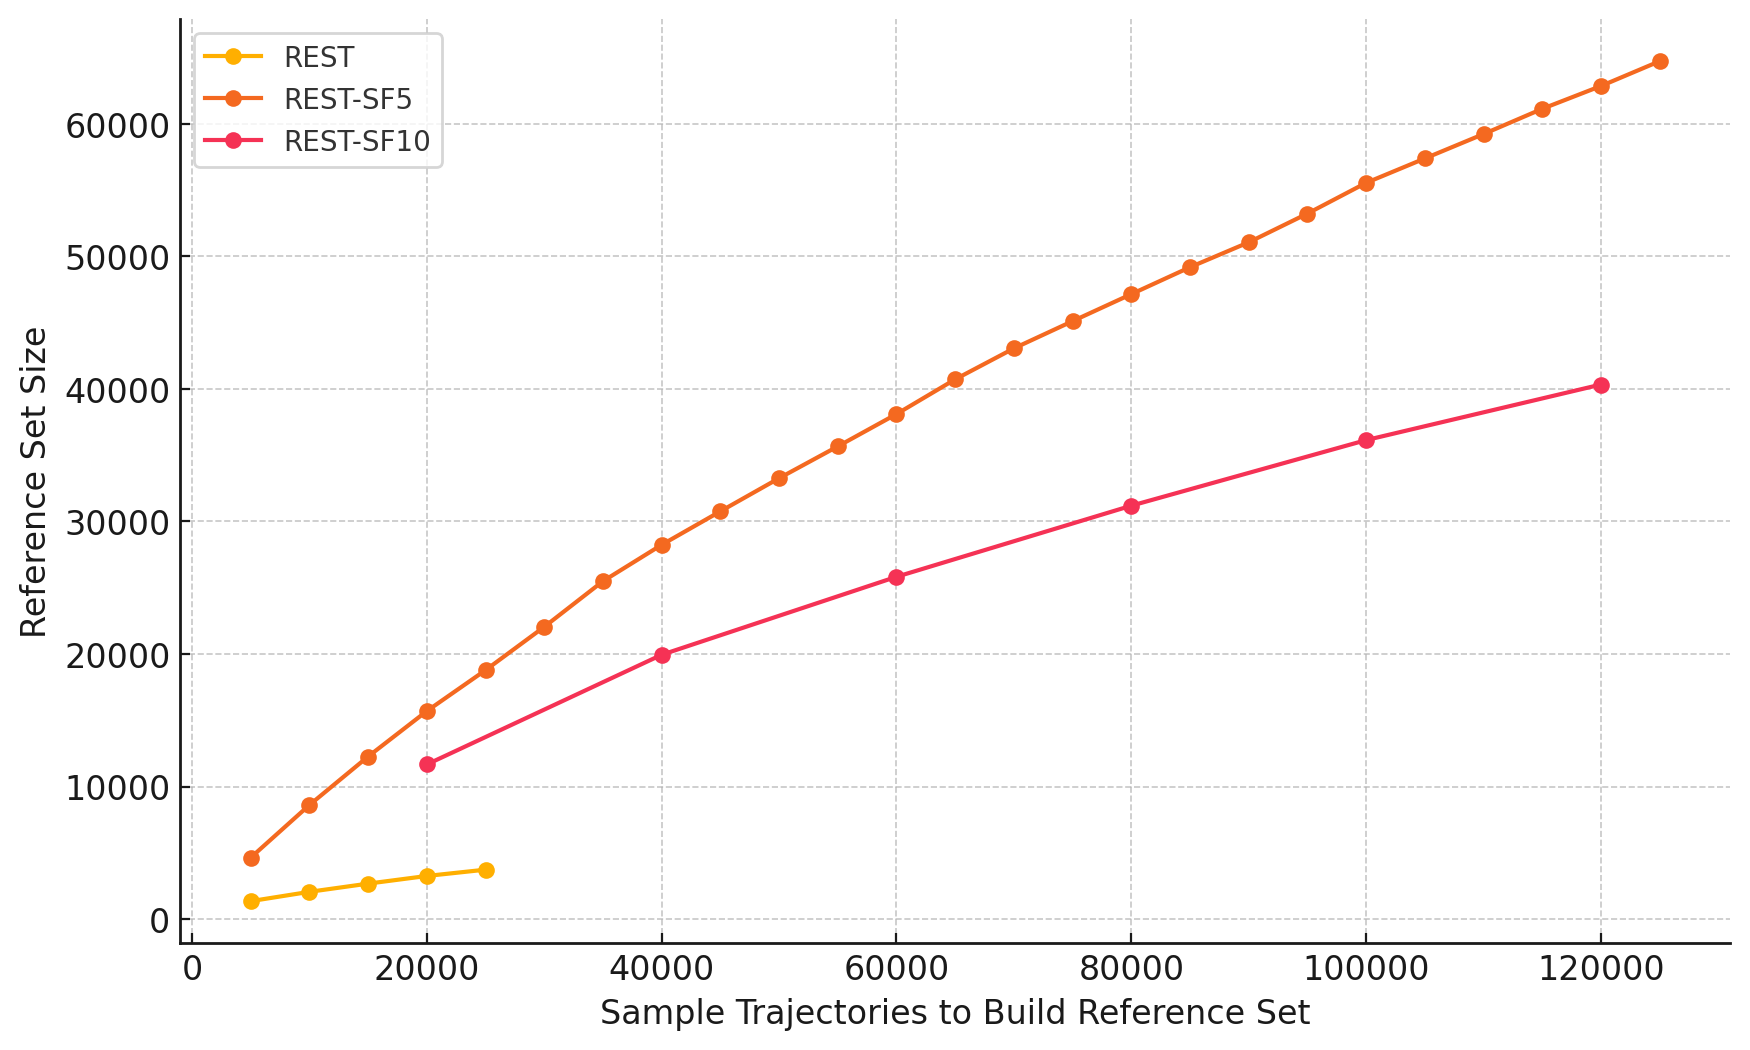
\includegraphics[height=8cm, keepaspectratio]{./figures/set_size.png}
        \caption{Reference set size over sample size. Each mode has a unique color}
        \label{fig:set_size}
    \end{minipage}
\end{figure}
\begin{figure}[h!]
    \begin{minipage}[b]{0.99\linewidth}
        \centering
        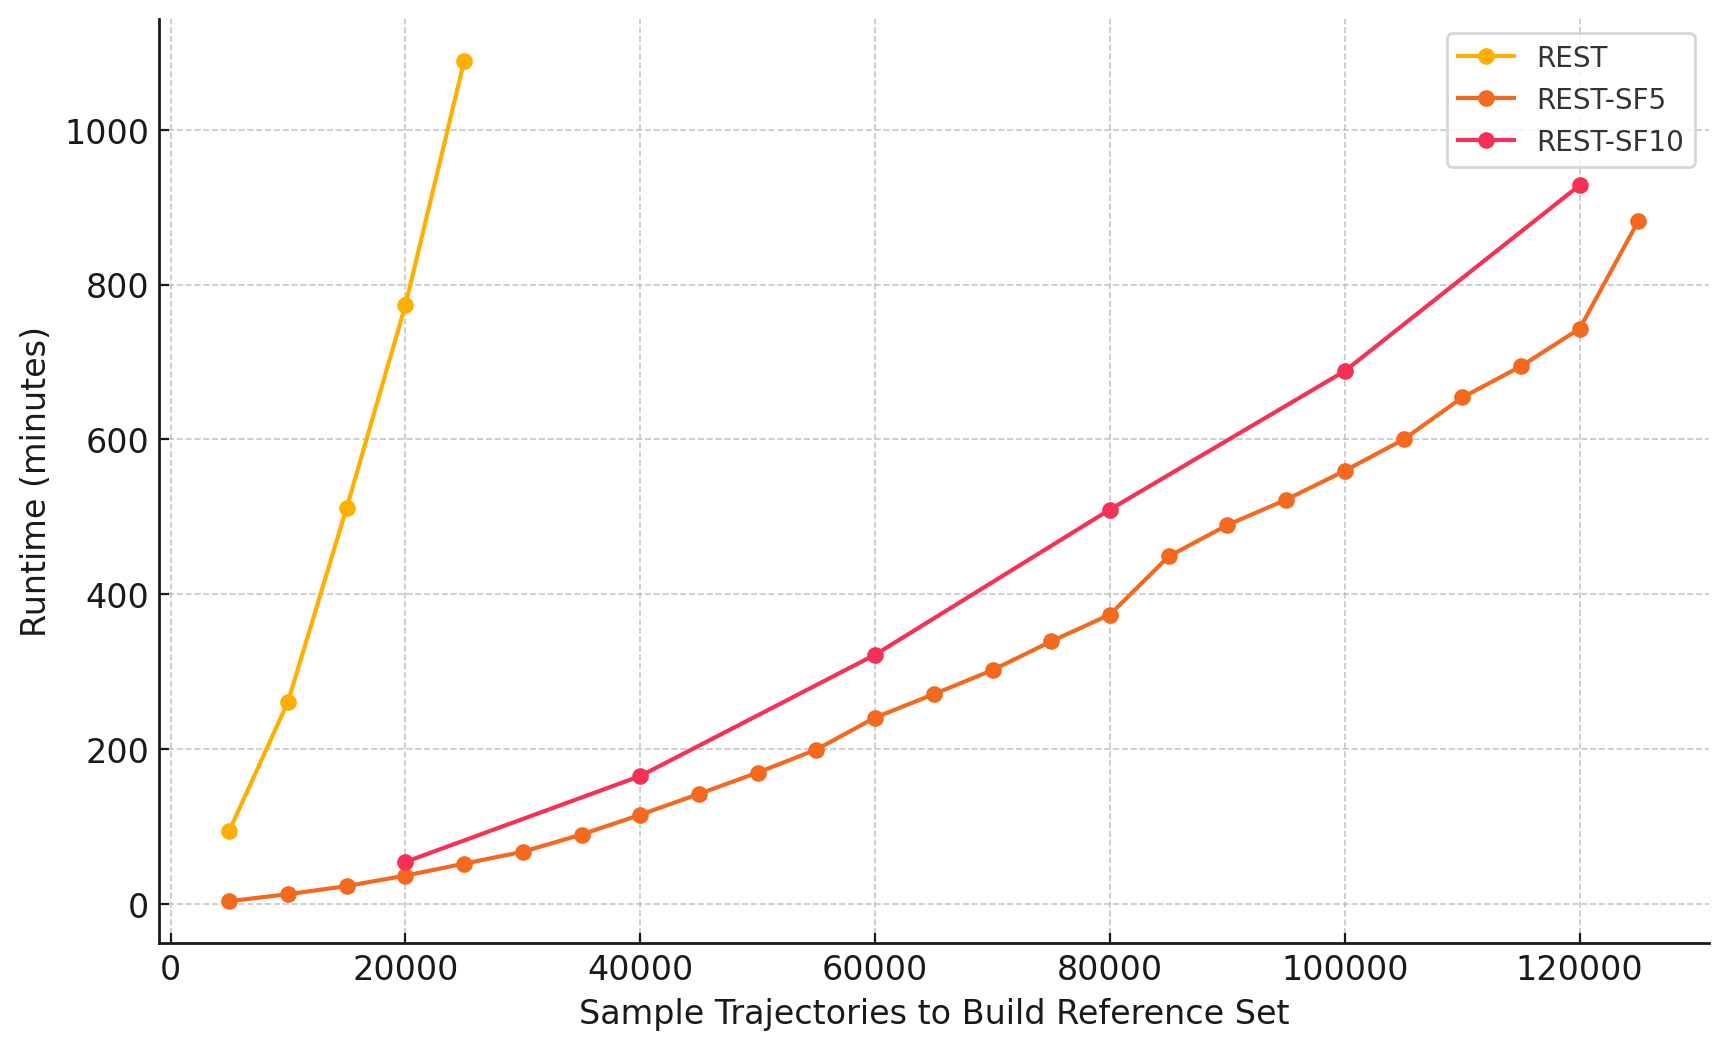
\includegraphics[height=8cm, keepaspectratio]{./figures/set_runtime.png}
        \caption{Reference set construction runtime over sample size. Each mode has a unique color}
        \label{fig:set_runtime}
    \end{minipage}
\end{figure}

In figure \ref{fig:set_size} we can see that \textit{REST} has a lower set size to sample size ratio, meaning it can represent a large sample with a small set. This must be considered the lower bound for sample size, since \textit{REST} can be seen as having an infinite window size, because it uses all reference trajectories. There is a trend that increasing window size approaches decreases set size, as we can see \textit{REST-SF75} is much lower in this regard than \textit{REST-SF15}. We also see that for all variants the growth in set size slowly decreases as sample size increases, this trend is also strongest for \textit{REST} closely followed by \textit{REST-SF75}. This might indicate the reference set size is approaching some finite value (converging) as the sample size increases. If the value converges, it makes a strong case for the effectiveness of reference based compression strategies in general. Intuitively this can be seen as the road network of a given city. If all the roads / routes have been mapped by the reference set then all new routes can also be represented by that.

For the runtime seen in \ref{fig:set_runtime} it is clear that \textit{REST} is much slower than the spatial filter variants. This is expected as it operates as if having an infinte window size, while \textit{REST-SF75} uses a $75\times75m^2$ window, significantly reducing the search space. There is a clear trend that increasing window size leads to increasing runtime. All in all, \textit{REST-SF75} seems to strike a balance between efficiency and maintaing a low sample size.
\section{Compression Performance}

\begin{figure}[ht]
    \begin{minipage}{0.99\linewidth}
        \centering
        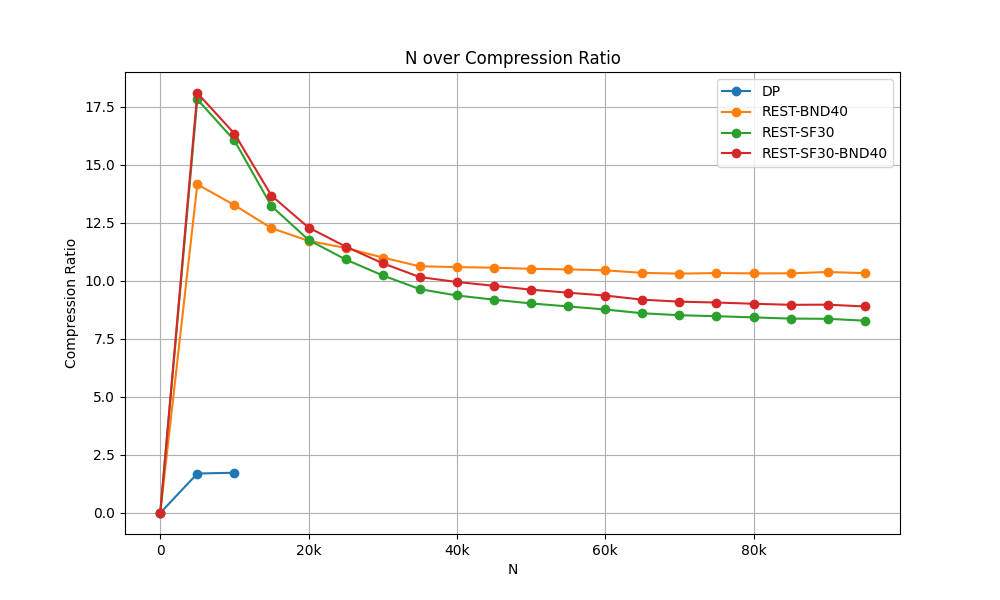
\includegraphics[height=8cm, keepaspectratio]{./figures/n_compression.png}
        \caption{N over compression ratio for a set sample size of 10k.}
        \label{fig:n_compression}
    \end{minipage}
\end{figure}
\begin{figure}[h!]
    \begin{minipage}{0.99\linewidth}
        \centering
        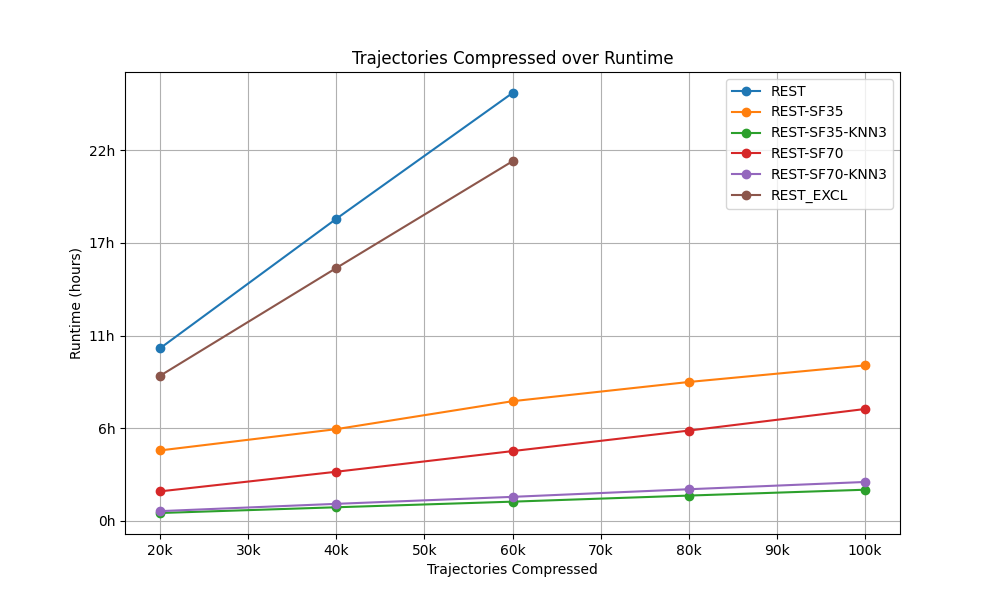
\includegraphics[height=8cm, keepaspectratio]{./figures/n_runtime.png}
        \caption{N over compression runtime, includes runtime for set construction with a sample size of 10k}
        \label{fig:n_runtime}
    \end{minipage}
\end{figure}
This section discusses the performance of the compression, using a reference set built from a sample size of 10k. $N$ represents the amount of compressed trajectories. Additionally we include experiments with the Sakoe-Chiba band, represented by BND in the graph label. The label \textit{REST-SF30-BND40} refers to a REST implementation that uses a spatial filter with a window size of 30 and a Sakoe-Chiba band size of 40. We also compare the different REST variants with Douglas-Peucker (DP). Figure \ref{fig:n_compression} show a clear spike in compression ratio at N = 10k for the REST variants. This is because many of the trajectories in the first 10k were added to the reference set and will have an exceptionally high compression ratio. Afterwards the compression ratio gradually falls, but stabilizes between 7.5-10.0. The compression ratio of DP is much lower, staying around a compression ratio of 2. The graph is cut off, however DP is expected to stay at the same level as N increases. this shows that REST significantly outperform DP.

However, note that the compression ratio for REST does not include the reference set size (this might change in future versions). This means that the real compression ratio will be lower, however considering the small size of the reference set compared to $N$, this is expected show promising results nonetheless.

With regards to runtime as seen in figure \ref{fig:n_runtime}, we see that all REST variations significantly outperform DP. When comparing REST variants we see that \textit{REST-SF30} is much faster than \textit{REST-BND40}. The combination of both strategies \textit{REST-SF30-BND40} only marginally outperforms \textit{REST-SF30}. This suggests that the spatial filter is most efficient speed up strategy, while the band only slightly improves performance. Looking at the differences between the two this indicates a bottle-neck for performance in REST. The spatial filter reduces the number of trajectory comparisons required, while the band decreases the runtime of each individual comparison. Thus, reducing the number of Dynamic Time Warping (DTW) distance calculations is a more efficient than speeding up individual calculations.
% \input{chapters/4-conclusion.tex}

\chapter*{\bibname}
\printbibliography[heading=none]

\input{chapters/papers.tex}

\appendix
\chapter{Additional Material}
\label{app:additional}

Additional material that does not fit in the main thesis but may still be relevant to share, e.g., raw data from experiments and surveys, code listings, additional plots, pre-project reports, project agreements, contracts, logs etc., can be put in appendices. Simply issue the command \texttt{\textbackslash appendix} in the main \texttt{.tex} file, and make one chapter per appendix.

If the appendix is in the form of a ready-made PDF file, it should be supported by a small descriptive text, and included using the \texttt{pdfpages} package. To illustrate how it works, a standard project agreement (for the IE faculty at NTNU in Gjøvik) is attached here. You would probably want the included PDF file to begin on an odd (right hand) page, which is achieved by using the \texttt{\textbackslash cleardoublepage} command immediately before the \texttt{\textbackslash includepdf[]\{\}} command. Use the option \texttt{[pages=-]} to include all pages of the PDF document, or, e.g., \texttt{[pages=2-4]} to include only the given page range.

\end{document}
